\documentclass[11pt,a4paper,titlepage]{report}

\usepackage{url}
\usepackage{csquotes}
\usepackage[backend=biber, style=trad-abbrv]{biblatex}
\usepackage{amsmath}
\usepackage{amssymb}
\usepackage{graphicx}
\usepackage{siunitx}
\usepackage{listings}
\lstset{frame=tb,
	language=c,
	aboveskip=3mm,
	belowskip=3mm,
	showstringspaces=false,
	columns=flexible,
	basicstyle={\small\ttfamily},
	numbers=left,
	breaklines=true,
	breakatwhitespace=true,
	tabsize=3
}

%opening
\title{Final Project: Draft Report}
\author{Richard Sefton}
\date{}

\usepackage{graphicx}
\graphicspath{{./assets/}}
\usepackage[inkscapeformat=png]{svg}

\addbibresource{BIBLIOGRAPHY.bib}

\begin{document}
	\maketitle	
	\tableofcontents
	
	\begin{abstract}
		\textit{
			This preliminary report focuses on the initial research into, and the making of a prototype of an Autonomous Underwater Vehicle (AUV) for the Final Project. The AUV will be written in primarily C code using bare metal AVR ATTiny1627 Microcontrollers and developed as independent modules networked using the $I^{2}C$ peripheral in a way that would make it extensible to accommodate various sensor payloads. An outline of the Minimum Viable Product for this project is a vehicle that is able to Autonomously drive itself through a body of water, avoiding obstacles, with additional features such as data transmission and following mission paths to be developed in phases once MVP has been reached.
		}
	\end{abstract}
	
	\chapter*{Introduction}
	\addcontentsline{toc}{chapter}{Introduction}
	
	For this project, I plan to develop an autonomous submarine or AUV (Autonomous Underwater Vehicle) as they are commonly known. AUVs are not a new or unexplored field. They have been produced since the 1950s with various examples at the commercial and research levels along with some parallels that can be drawn in the amateur space with remote control submarine projects. 
	
	This project was born from a personal enjoyment of the Internet of Things module which allowed me to explore microcontroller programming, and interacting with physical electronic sensors and actuators. This blossomed into a passion for robotics, and as one of the early module videos highlighted our projects should be something we are passionate about: without passion, we would be unmotivated to complete this lengthy and isolated piece of work \cite{COURSERA_PROJECT_VIDEO}. This project does not comfortably fit within any of the given templates - I found the templates for Internet of Things were topics I'm not passionate about. I did gain permission for this idea via the Coursera forums\cite{COURSERA_PROJECT_PERMISSION} prior to embarking on this journey. Screenshots of the permission can be found in the images \ref{picture:permission_1} and \ref{picture:permission_2} of Appendix \ref{appendix:project_permission}.

	The inspiration for this project came from various YouTube videos by a single YouTuber (Brick Experiment Channel\cite{BRICK_EXPERIMENT_CHANNEL_PROFILE}) whereby the person created iterative versions of a remote controlled submarine using a watertight container and Lego. While these videos and their associated blog\cite{BRICK_EXPERIMENT_CHANNEL_BLOG} serves as the initial inspiration, the idea to automate it comes from a fascination with robotics. 
	
	\section*{Previous Works}
	\addcontentsline{toc}{section}{Previous Works}
	\subsection*{Amateur Level}
	\addcontentsline{toc}{subsection}{Amateur Level}
	The YouTuber Brick Experiment Channel\cite{BRICK_EXPERIMENT_CHANNEL_PROFILE} wrote a series of blog posts\cite{BRICK_EXPERIMENT_CHANNEL_BLOG} outlining the build process for the $4^{th}$ iteration of their remote controlled submarine. 
	
	The posts are detailed covering the steps of building this submarine with reasoning behind the design decisions along with a critical evaluation of each step. This version is using a large syringe to bring water onboard the vehicle to control buoyancy, and is driven by two motors: one for propulsion, and one for direction. The sensors incorporated measure pressure to accurately gauge depth, and a laser to measure distance from the bed of a body of water. 
		
	The blog also raised communication as a consideration: While the aim of this project is to build an autonomous vehicle, it would be nice to communicate with it in flight. The problem is this cannot be done easily with wireless frequencies as the higher frequencies that provide the required bandwidth do not penetrate water that well.
	
	\subsection*{Commercial Level}
	\addcontentsline{toc}{subsection}{Commercial Level}
	The company Advanced Navigation makes the Hydrus Drone\cite{ADVANCED_NAVIGATION_HYDRUS}, which claims to be one of the smallest AUVs on the market. The device itself controls depth and position with impellers, a 4K camera with AI integrations, and a forward facing sonar. The most important aspect of Advanced Navigation's AUV is how they address the issues around wireless communication. This company has fitted their device with acoustic and optical modems so data can be transferred using audio frequencies and light (presumably similar to fibre octics).
	
	\subsection*{Research Level}
	\addcontentsline{toc}{subsection}{Research Level}
	The Woods Hole Oceanographic Institute\cite{WOODS_HOLE} draws attention to the use of different AUVs depending on the area of research or environment. They use one of 6 AUV models, which operate at different depths or different functionality.The REMUS\cite{WOODS_HOLE_REMUS} can be equipped with varying sensors and is programmed for survey missions. It was adapted to survey the Delaware river Aqueduct for leaks. 
	
	One of the more interesting AUVs this institute uses is the Spray Glider\cite{WOODS_HOLE_SPRAY_GLIDER}. This description for this device is one that glides through the water without any external thrusters so can be travel for weeks at a time. The device uses internal bladders to control buoyancy, and is set to navigate preset paths equipped with varying sensors. What is interesting about this device is the lack of external propulsion seems to make this device more passive, and can therefore operate at lower voltage.
	
	The UK National Oceanography Centre has details on the challenges around an designing an AUV\cite{NATIONAL_OCEANOGRAPHIC_AUTOSUBS}. For power and propulsion it highlights the lack of oxygen for internal combustion makes it necessary to use batteries for power and notes the difference in speed between AUVs and surface ships. For navigation it highlights that because GPS can't penetrate the top few mm of water, the reliance on other techniques is required. It suggests an approach called Dead Reckoning which gets the speed of the AUV by measuring the Doppler shift from the sea bed for relative speed and using a gyro to measure the heading. It highlights that navigational accuracy is vital to survey missions. 
	
	\chapter*{Literature Review}
	\addcontentsline{toc}{chapter}{Literature Review}
	The definition for an AUV is best described in an article titled "Autonomous Underwater Vehicles (AUVs): Their past, present and future contributions to the advancement of marine geoscience". 
	
	\begin{quote}
		Autonomous Underwater Vehicles (AUVs) are unmanned, self-propelled vehicles that are typically deployed from a surface vessel, and can operate independently of that vessel for periods of a few h to several days.\cite{AUV_PPF}
	\end{quote}
	
	The authors go on to highlight that "In addition, recent economic drivers, such as rapidly increasing vessel fuel oil costs, are making autonomous systems a potentially attractive proposition to organisations responsible for large-scale and cost-effective marine data collection programmes"\cite{AUV_PPF}. This article addresses the commercial benefits of AUV production and deployment but doesn't address the human benefits such as safety. 
	
	The authors also discuss the applications of AUVs and point out that "the sensors deployed determine the vehicle altitude, as well as its speed and endurance."\cite{AUV_PPF} The endurance in this context is the available power to the AUV which would affect its overall range. Because different sensors and actuators have varying power requirements, some of these components may draw more power than others. The array of sensors required is defined by the AUVs use case: it would be inefficient mounting water quality sensors onto an AUV designed for ocean bed mapping survey. 
	
	While this article includes a lot of jargon relating to marine geosciences, it provides a good overview of the uses of AUVs and their previous applications. More importantly, it provides some good starting points for some concepts I will need to  explore during the development of this project. This includes references to works that look into the Dead Reckoning method of positioning, and a launch pad into some key concepts such as Sonar. 
	
	\section*{Communication}
	\addcontentsline{toc}{section}{Communication}
	Because the sensors deployed on an AUV are specific to its function and is something that can be configured, it is worth considering a modular design. As a part of this there could be some level of connectivity between the separate modules. Modern MCUs typically feature multiple options for communication protocols such as UART, USART, $I^{2}C$, SPI, USB, Ethernet or could be as simple as pulling a pin high or low. For the purpose of this project, we will consider $I^{2}C$ as it uses minimal wires, and allows for two way communication. The MCU data sheet\cite{ATTINY1627} is the manufacturers documentation and is a vital reference for development on any given  MCU and it directly relates to the MCU specific library in code. It has all the details and requirements to setup any of the provided MCU features, and gives a brief overview of each feature. 
	
	With regards to the ATTiny 1627 MCU, the data sheet describes $I^{2}C$ as a TWI (Two Wire Interface): "The Two-Wire Interface (TWI) is a bidirectional, two-wire communication interface (bus) with a Serial Data Line (SDA) and a Serial Clock Line (SCL)"\cite{ATTINY1627}. There are several advantages to using the TWI bus as a communication protocol as it allows the connection of "one or several slave devices to one or several master devices"\cite{ATTINY1627} allowing a network of devices to become interconnected. This would also allow for parallel computation as instead leaving one device to perform all of the sensor readings and calculations, some of which could be computationally expensive or using deliberate pauses of code execution, a master device could simply trigger the networked modules to each perform their actions and then do nothing while waiting for the responses. 
	
	In the article 'FEATURES, OPERATION PRINCIPLE AND LIMITS OF SPI AND $I^{2}C$ COMMUNICATION PROTOCOLS FOR SMART OBJECTS' the authors share their opinion on how an IoT network should operate and how it should be secured, and then give an overview of both $I^{2}C$ and SPI protocols before suggesting a hybrid version of the two. For IoT networks the authors suggest that "different devices with different capabilities will take part in the creation of a network. A self-describing interface for each device is necessary in order to optimize the management of required tasks"\cite{I2C}. This point backs up my idea of a modular design where sensor modules can be attached in a way to form a network where each module is responsible for a specific task. They then go on to highlight that "adding an object to the network should not cause the collapse of the network itself. The network should also properly handle the failure of a device"\cite{I2C}. This point involves error handling within a network of discreet modules. If one module fails, the whole unit should not. If the module is deemed vital to the devices operation, such as obstacle avoidance sensors on an AUV, a graceful way to handle this could be to surface the device and broadcast a signal indicating the error on a predefined wavelength so it can be collected. 
	
	For $I^{2}C$ the authors give a detailed overview stating that:
	
	\begin{quote}
		The \textit{Inter Integrated Circuit} ($I^{2}C$) protocol, ..., was developed by Philips in 1982 and it is a serial, single-ended bus with multi-master support and typically used to connect low speed devices.\cite{I2C}
	\end{quote}
	
	The bandwidth available over the standard $I^{2}C$ rail is slow at 100\unit{\kilo\bit}/\unit{\second}, but there is a Fast mode and Fast Plus mode which allows up to 1\unit{\mega\bit}/\unit{\second}. Additionally some devices also support a high speed mode which allows up to 3.4\unit{\mega\bit}/\unit{\second}.\cite{I2C_FAST}. This means the $I^{2}C$ rail may not be suitable for \textit{all} types of sensors attached, particularly ones that gather a lot of data in real time, for example high definition cameras. 
	
	\begin{quote}
		Since the bus is completely shared, it is possible, for devices, to receive not only unicast transmission but also broadcast messages: for this reason, whenever master wants to write or read data from a particular slave, it will address it first. Addressing bits were originally seven, extended to 10 with the latest reviews to increase supported maximum number of connected devices. $I^{2}C$ bus supports multiple masters on the same bus too, but a proper conflict-solving algorithm has to be implemented. \cite{I2C}
	\end{quote}
	
	This addressing is how the devices know what devices they need to talk to on a network. With the system of addressing and the ability to broadcast transmissions we can begin to visualise the $I^{2}C$ protocol as akin to web sockets. The interesting point raised here is that conflict resolution needs to be handled where the network has multiple masters. One such proposal they put forward is Arbitration: "since $I^{2}C$ supports multiple masters, an arbitration rule is necessary. In this protocol, arbitration proceeds bit by bit and the rule is deterministic: the first master that produces a one when the other produces a zero loses the arbitration"\cite{I2C}. 
	
	Another resource that covers a lot of information about AVR Microcontrollers and also providing an overview of the features as well as how to interact with actuators such as servos and stepper motors, is 'Make: AVR Programming'\cite{MAKE_AVR}. While this book does contain quite a broad overview of the features and protocols, it also has examples of code to interact with them, as well as an overview of the toolchain required to programme a microcontroller (in this instance involving Make, avr-gcc\cite{GCC_AVR} and AVRDude\cite{AVRDUDE} as well as a physical hardware programmer). However, the example code is all written for a specific MCU that the book focuses on, being the ATMEGA168. However, as the author notes, this should not be too difficult to port to my specifically chosen MCU as the book also tries to teach another skill being the ability to refer to relevant sections of the data sheet. 
	
	As well as internal device communication protocols, it would also be good if we could have some way of interacting with the device in flight: receiving data, and possibly some rudimentary manual over ride/remote control. As corroborated in an article exploring underwater wireless networks, "radio is seriously attenuated in water"\cite{UNDERWATER_RADIO}. Radio waves exist on the EM Spectrum and the lower the frequency, the further it can penetrate water due to the electrical dissipation that occurs, which is accentuated by salt water. High frequencies that we are used to as standard data transfer frequencies (WiFi, Bluetooth) are measured in \unit{\giga\hertz}, and these penetrate only a few \unit{\centi\meter} of water. Even LoRa at 433\unit{\mega\hertz} will only penetrate 30-50\unit{\centi\meter} of water. The military use lower radio frequencies operating in the range of \unit{\hertz} to \unit{\kilo\hertz} to communicate with their submarines but the trade off is lower frequencies bandwidth (less data can be transferred as there are fewer cycles per second). Additionally, radio frequencies are controlled\cite{RADIO_FREQ_TABLE} and as a hobby enthusiast/student I only have access to a limited range of frequencies.  
	
	The article also states "acoustic communication is almost the only effective way for underwater wireless transmission. Nevertheless, compared with the traditional radio, underwater acoustic communication is greatly affected by poor conditions, such as absorption, scattering, multipath interference and Doppler effect"\cite{UNDERWATER_RADIO}. While I think the authors are perhaps exaggerating this point to justify their experiments somewhat, it does offer an alternate avenue to wireless communication with a device while it is operating underwater, but it would require the development of an ultrasonic modem of some description. Alternatively we could just add a plug to the device for a physical wire for external control/data transmission. While this goes against the design of an AUV as being untethered, it would also act as a lifeline to retrieve the device while minimising risk, even when testing in controlled bodies of water. 
	
	\section*{Navigation}
	\addcontentsline{toc}{section}{Navigation}
	
	Since AUVs are unmanned, they require a method of obstacle avoidance. Above water levels, using air as the medium there are several options available such as ultrasonic range finding, lasers or LiDAR devices, Radar, machine vision (aided with cameras), or radio signal strength to avoid obstacles such as similar devices that are networked. When the environment changes, the methods become more restricted: ultrasonic range finding is not an option in the vacuum of space as it requires a medium for the sound waves to travel through. In the case of underwater, most of the options listed above \textit{can} work under certain conditions. Machine vision using cameras for example can work in clear waters. Once the water becomes murky or turbulence occurs the images can become distorted or the effective range is reduced. Lasers have a similar issue where the refraction of light in the water makes it difficult to use this as an accurate gauge. Of all the options, Ultrasonic range finding is one of the few consistently viable options for consistently accurate measurements. When used underwater, Ultrasonic range finding becomes Sonar. 'A Brief History of Active Sonar' while discussing the threat of submarines during WW1 states that:
	
	\begin{quote}
		Since sound is the only transmitted energy that penetrates water for any appreciable distance, acoustic echo-ranging had to be exploited to counter this threat. \cite{ACTIVESONAR_HISTORY}
	\end{quote}
	
	the technology was developed by Reginald A Fessenden. "In a response to the need for enhanced detection of submerged objects and enemies, the first successful underwater transducer developed was a 540-\unit{\hertz} electrodynamically driven circular plate"\cite{ACTIVESONAR_HISTORY} and "the use of the word \textit{sonar} for these systems, defined as Sounding Navigation and Ranging, was coined in 1942 by F. V. Test Hunt, director of the Harvard Underwater Sound Laboratory" \cite{ACTIVESONAR_HISTORY}. A transducer is an electrical component that can emit sound waves in a set frequency. Additionally, the transducer can \textit{detect} sound waves on the same resonant frequency. When the detection occurs the sound waves cause the transducer to vibrate generating an electrical signal \cite{TRANSDUCER_YOUTUBE}.
	
	\begin{quote}
		The inter-war period was also a time for basic research in underwater acoustics. One key discovery during this period was that amplitude of higher frequencies of underwater sound are attenuated more than lower frequencies as they pass through the seawater. \cite{ACTIVESONAR_HISTORY}
	\end{quote}
	
	This observation states that lower frequencies penetrate water better than the higher frequencies, i.e. lower frequencies provide a longer range, but what this article fails to cover is that higher frequencies provide a higher resolution when it comes to sonar imaging technology \cite{HF_SONAR}.
	
	\chapter*{Project Design}
	\addcontentsline{toc}{chapter}{Project Design} 
	
	\section*{Domain}
	\addcontentsline{toc}{section}{Domain}
	AUVs have applications spanning multiple domains both in scientific exploration as well as commercial enterprise. For science they are used for surveying coastlines and ocean beds, sampling in remote or hard to reach locations and exploring the depths to name a few applications. For commerce they can de deployed to monitor gas and oil pipelines, monitor drills, survey potential resource sites, and monitor ship hulls etc. The deployment of AUVs over physical diving or manned equipment offer more benefits when compared to the cost. AUVs can potentially spend longer underwater depending on the design and payload they are equipped with and the size of the power source, and can gather far more data than a diver with far less risk to human life (if they are deployed at sea the risk will never be zero, but there is considerably less \textit{additional} risk).
	
	For the purposes of this project the AUV I will develop will be targeted towards the scientific exploration domain, specifically those designed for survey missions. AUVs in this domain are highly configurable with the payload (being the array of sensors attached) being customised for the survey being conducted, often with fallback sensors to verify the data (such as cameras coupled with sonar), or designed from the ground up for a specific operational area. This project will be focused on a customisable AUV focusing on the core mechanics that make it autonomous. The minimal viable product for this project is going to offer basic functionality (object avoidance primarily), but will be modular in design. The sonar and motor controllers would be separate Client modules bound by a central Host MCU. 
	
	\section*{Technologies}
	\addcontentsline{toc}{section}{Technologies}
	For this project I plan to use predominantly AVR based microcontrollers with code written in C using the official AVR libraries, but otherwise a "bare metal" approach. This project will be using little to no Arduino code as now is a good learning opportunity to programme microcontrollers without relying the Arduino layer of abstraction or the on board programmer attached to a pre-fabricated Arduino boards. Additionally, by focusing on the MCU alone, PCBs can be fabricated for this project with a far lower footprint than trying to fit in multiple individual Arduino boards, which could prove invaluable if space and weight becomes a premium. The specific MCU I plan to use is the AVR ATTiny1627\cite{ATTINY1627} due to its small size and power requirements. The device can operate on 1.8\unit{\volt} to 5.5\unit{\volt} making it potentially extremely low powered, and is also feature rich (Appendix \ref{appendix:attiny_features}).
	
	Unfortunately the chip itself is extremely small as the 24 pin 1627 is only available in QFN (or VQFN packaging), which is incompatible with a breadboard for development and testing. To mitigate this I have developed a QFN breakout board (Appendix \ref{appendix:vqfn_breakout}). This has proven to be economically viable as the cost per board was only £7 and the MCU was less than £1 making the per board cost for each MCU to be < £8. This comparable with the Raspberry Pi Pico or the NodeMCU 8266\cite{8266} and significantly cheaper than the Arduino Uno or larger Raspberry Pi models. 
	
	The AUV itself will be using predominantly large diameter plastic tubing or a suitable size plastic tub along with various adhesives and sealants (silicone based) for waterproofing the device. Lego will also be used for structural support and for aiding in the various mechanisms to drive the device (such as rotors/propellers). The use of Lego has been decided over creating custom devices on a 3D printer due to budget and time constraints.
	
	For navigation and obstacle avoidance this project will employ the use of sonar. While prefabricated sonar units designed for underwater applications exist, these are often expensive with devices such as the Ping2 by Blue Robotics\cite{PING2} which is designed for this type of application starting from ~£400. While devices such as this are extremely feature rich, they are out of reach for this project. Alternatively there are various fish finders on the market that start from ~£40 which could be hacked to become compatible with this project. There is also the option to use the HC-SR04\cite{HC-SR04} ultrasonic rangefinders, but they may not be suitable for this application for a few reasons:
	\begin{itemize}
		\item The HC-SR04 is not designed for underwater applications. There may be an issue with the air gap between the transducer itself and the hull of the vessel which in itself could be problematic. The transducers may have to be mounted outside of the vessel. 
		\item The HC-SR04 is primarily designed for over the air applications. Speed of sound travels faster through water than in the air and the MCU that is controlling the device may be tuned to enable the receiving transducer only after set time period to reduce false positives and noise. This period would shorten the minimum range of the sensor. 
	\end{itemize} 
	
	For these reasons I will aim to develop a sonar module from scratch. The data sheet for the HC-SR04 module is also quite useful as it provides a formula for calculating distance in the air.
	
	$$
	Range=\frac{High Level Time \times Velocity}{2}
	$$\cite{HC-SR04}
	
	In this formula, Velocity is the speed of sound. The data sheet describes this as a flat 340\unit{\meter}/\unit{\second} which is slightly inaccurate. The speed of sound is impacted by environmental factors such as temperature, humidity and the transmission medium meaning the Velocity would need to be adjusted for water, and saltwater more so\cite{SOS_CALC}. Another article, titled 'Design and Development of an Ultrasonic Motion Detector'\cite{USONIC_MOTION_DET} could prove to be valuable to this project as it covers the development process in creating an ultrasonic device to detect motion. While this is not fully what I will be looking to accomplish, it provides insight on two key concepts: A Sonar circuit diagram example, and Doppler Shift which is used in Dead Reckoning to help provide the speed of the AUV relative to a fixed point. 
	 
	For propulsion the plan is to use either a toy motor or a stepper motor. The toy motors are easier to drive, using Pulse Width Modulation fed into a prefabricated driver circuit to specify the speed. The issue with the toy motor however is the torque - it may not have the required torque to drive a shaft as the current plan is to use magnets to connect an internal and external shaft in the same way as the YouTuber "Brick Experiment Channel"\cite{BRICK_EXPERIMENT_CHANNEL_BLOG}. The stepper motor will provide the required torque but speed adjustment is not quite as simple as modifying the PWM duty cycles.
	
	For depth control the plan is to use a large syringe similar to "Brick Experiment Channel" RC Submarine but this will involve some experimentation to see if this can be achieved by modifying the weight of the vessel by taking on water from outside, or by changing the density of the vessel by compressing the available air. The syringe will be driven by a motor, which will likely be a stepper motor given the compression and decompression will require more torque than the toy motors can provide and because this requires somewhat more precision. This will also require a method to convert the rotary force to a linear push/pull force on the syringe plunger. 
	
	
	\section*{Project Plan}
	\addcontentsline{toc}{section}{Project Plan}
	
	This is a highly ambitious project. For this reason it is necessary to outline a clear minimum viable product, with phased further development beyond this point. The MVP will consist of the core components that will make an AUV able to move through a body of water:
	
	\begin{itemize}
		\item Propulsion
		\item Directional control
		\item Depth Control
		\item Sonar for obstacle avoidance
		\item Main control unit to gather sonar data and respond to external influence (directional control and driving) - In short, Autonomy.
	\end{itemize}
	
	The MVP for this project will be broken down to its core modules and developed as discreet entities. For example the sonar module would be a module that sits on the $I^{2}C$ rail and performs on receiving a command returning the distance to the requester. By splitting the development into modules, the development can be easily broken down to follow a more Agile method of development where the modules can be developed and integrated into the final product in sprints. The modular design will also allow the easy integration of multiple of the same modules: if it becomes apparent that more sonar is required, we can simply add another to the $I^{2}C$ with minimal changes to the controlling module. 
	
	Phase 2 of this project will involve expanding on the MVP to include the following features:
	
	\begin{itemize}
		\item Algorithm for surfacing and data transmission.
		\item Configured WiFi device (8266) to transmit the data
		\item Companion app to receive and visualise the data
	\end{itemize}
	
	Phase 3 of this project will involve expanding on Phase 2 to include the following feature:
	\begin{itemize}
		\item Use of Dead Reckoning to obtain relative speed of the vessel
		\item Integration of a gyro to gauge an accurate heading
		\item Programming interface to upload a planned path
		\item Algorithms to follow the path, correcting for unknown obstacles along the way
	\end{itemize}
	
	The project has been planned with the aid of GitHub Projects\cite{GITHUB_PROJECTS_DOCUMENTATION}. The details of the project planning can be found in \ref{appendix:project_plan} of the Appendix, and the GitHub repository is referenced in the bibliography. \cite{GITHUB_REPO} \cite{GITHUB_PROJECT}. The repository should be public, but the project itself may be private and inaccessible. Going by the project plan I am currently behind schedule owing to issues discovered building a working Sonar module from scratch, but this is the last component required to get working before MVP can be achieved so I am not overly concerned right now. 
	
	\section*{Evaluation Plan}
	\addcontentsline{toc}{section}{Evaluation Plan}
	For the MVP of this project, the plan is to test each module in isolation before bringing them all together. The testing will primarily be done outside of the water, with calculations for the sonar tuned to over the air transmission and reception, with the objective to modify this small part prior to testing in the water. Using the RTC peripheral with a high frequency clock provides the requisite resolution to calculate underwater so this approach should work. Testing in water will only be done at the end of the project once a complete device has been created and can be verified to be water proof, as even with low voltages I lack the expertise to comfortably and safely test with water.
	
	The acceptance criteria for a successful evaluation for the MVP once it has been accomplished will be a device that when in a body of water will be able to move autonomously in any direction, avoiding obstacles. There are ethical concerns surrounding wildlife that could be affected: ultrasonic is outside the range of human hearing, but even if wildlife can't hear ultrasonic sound waves, there are other considerations such as failed tests causing injury to wildlife, or issues surrounding encroaching on territory and wildlife gaining injuries by attacking the AUV. To mitigate these concerns, the AUV will only be tested in small controllable bodies of water where no wildlife is present. The ideal solution would be a large swimming pool but this may not be an option due to availability or cost in renting a public pool for any period of time. Testing may have to be done in a smaller pool that can be erected and filled for testing purposes and relatively inexpensive depending on its capacity. A valid pool for testing would be one that allows testing of both navigation and depth control so it would need to be at least 1\unit{\meter} in depth. 
	
	\chapter*{Feature Prototype}
	\addcontentsline{toc}{chapter}{Feature Prototype}
	
	\section*{Overview}
	\addcontentsline{toc}{section}{Overview}
	For this stage in the project I have developed a prototype as a proof of concept of the modular design of each of the feature components. This prototype consists of 3 different modules:
	\begin{itemize}
		\item Sonar
		\item Motor Controller
		\item Central Controller
	\end{itemize}
	
	The modules are all networked using the $I^{2}C$ protocol using the AVR TWI peripheral using a star network topology where the Sonar and Motor Controller modules are each connected to the Central Controller with a Hos -> Client or Master -> Slave relationship, with the Central Controller acting as the Host/Master. The Central Controller is configured to perform the same action every second. This is accomplished using the Real Time Counter setup to trigger an event every second using the Overflow Interrupt which uses $I^{2}C$ to retrieve a distance from the Sonar Module, and depending on the data sent from the Sonar module will then issue an instruction to the Motor Controller module to either start or stop the motor, again using $I^{2}C$. The Sonar module is also using the RTC peripheral to time the delay between triggering the ultrasonic and receiving the response then calculates the distance before sending back the result. The Motor Controller module drives a motor in the main loop, controlled by a global variable adjusted depending on the value of the command received from the Central Controller module.  
	
	\begin{enumerate}
		\item Device powers on
		\item Module peripherals setup
		\item Modules enter infinite loop
		\begin{enumerate}
			\item \textbf{Controller}: RTC Interrupt event
			\item \textbf{Controller}: RTC issues $I^{2}C$ read operation to the \textbf{Sonar} module and enters a waiting state for the response
			\item \textbf{Sonar}: $I^{2}C$ Interrupt event fires
			\item \textbf{Sonar}: start time recorded from the RTC count buffer
			\item \textbf{Sonar}: HC-SR04 trigger pin pulled high for 10\unit{\micro\second}
			\item \textbf{Sonar}: Module waits for echo pin to fall low
			\item \textbf{Sonar}: Module gets the end time from the RTC count buffer and calculates the distance
			\item \textbf{Sonar}: Module sends data back to the \textbf{Controller} over $I^{2}C$
			\item \textbf{Controller}: Module uses the distance response to send either a start or stop command to the \textbf{Motor Controller}
			\item \textbf{Motor Controller}: Module receives a command to either start or stop the motor. $I^{2}C$ interrupt updates the global variable controlling the motor
			\item \textbf{Motor Controller}: Motor is driven by pulling pins connected to a motor driver high or low in a specific order
		\end{enumerate}
	\end{enumerate}
	
	The full code for this can be found in Appendix \ref{appendix:prototype_module_code} and \ref{appendix:twi_library}.
	
	\section*{Challenges}
	\addcontentsline{toc}{section}{Challenges}
	While the prototype concept is quite a simple one, the decision to not use Arduino code to facilitate this made it much harder to build. There were a couple of challenges in making this prototype that needed to be overcome or a compromise devised. First was with the Sonar module. The original plan was to build my own Sonar module that functions similarly to the popular HC-SR04\cite{HC-SR04} prefabricated ultrasonic range finder. This module uses inexpensive 40\unit{\kilo\hertz} transducers to emit a signal pulse using a Pulse Width Modulation signal of the same frequency connected to a MOSFET with a power source 12\unit{\volt} from a DC voltage step up circuit. The theory is the emitting transducer will emit a pulse which when bouncing off an object will cause the receiving transducer to oscillate at the same frequency generating an electrical signal. The received signal is amplified as the voltage would be quite small, and the time between starting the transmitter and receiving the response would be used to calculate the distance. In practice, this is not what is happening. The distance in my module is currently always returning the same value. At this stage I do not have any concrete reason why this is occurring but speculating I have a couple of ideas. First, it is possible that the voltage driving the transducers is not high enough. I have two different varieties of transducers: plastic ones\cite{PLASTIC_TRANSDUCER} similar to the HC-SR04, and Aluminium ones\cite{ALUMINIUM_TRANSDUCER} which are more waterproof. When integrating the Aluminium ones into this module absolutely nothing happens. The data sheet for the Aluminium transducers indicates that the maximum voltage is 160\unit{\volt} and 12\unit{\volt} source is not even 10\unit{\percent} of this. The plastic transducers have no maximum voltage in the data sheet but appears to work. The issue with the device always displaying the same distance value could be the receiving transducer is picking up the resonance from the transmitter while it is transmitting. As a compromise to build the prototype in time for this submission, I made this Sonar module using the HC-SR04\cite{HC-SR04}. The schematics for my Sonar module in its current state can be found in Appendix \ref{appendix:sonar_schematics}
	
	The second challenge faced during the development of this prototype was surrounding the $I^{2}C$ protocol. Using Arduino, there is easy access to the "Wire" class which initialises the protocol and supplies functions to send and receive data. The choice to use the bare metal approach meant I do not have access to such libraries. This meant that I needed to create my own library in order to use this feature, which I managed to do using a combination of the MCU data sheet\cite{ATTINY1627} and the Make: AVR Programming book\cite{MAKE_AVR}. The way the protocol works is the Host is configured with a baud rate to set the clock and the Client devices are initialised with an Address. The Host makes a request to a Client by sending the Client Address along with a bit indicating the mode of operation (Read or Write). 
	
	For write operations, the Client must respond with an acknowledgement that the address is correct. Once the Host has received acknowledgement (ACK) the clock (SCL) is held low and the bus is set to a busy state. The host can then send data. Each time the Client reads from the data buffer it can send the (ACK). If the Client can no longer receive data, it will send a not acknowledged bit (NACK). At this point the Host can send the stop command. Once the stop command is issued the bus state is set back to Idle where it is ready for the next command. Read operations are similar to this, with the exceptions that the Client device is handed control of the SCL and the Host must issue the ACK or NACK bits as well as the stop command. 
	
	Luckily, the ACK and NACK bits are handled automatically if "Smart Mode" is enabled on the peripheral which will automatically send these bits when the data buffers are read from or written to, or when the Interrupt flags are cleared. The main challenge faced developing this library was surrounding the stop command being issued incorrectly, which was either leaving the bus in an error state. This caused the protocol to hang after successfully sending the first request, or caused the Central Controller module to reset itself. This was eventually overcome after discovering\cite{MICROCHIP_TWI} that the stop command should be sent before writing to or reading from the data buffer. Once this was discovered, the stop command successfully put the bus state to idle when ending an operation, ready for the next. 
	
	\section*{Further Development}
	\addcontentsline{toc}{section}{Further Development}
	The next stage of development following on from this prototype is to get a working sonar module using the waterproof transducers\cite{ALUMINIUM_TRANSDUCER}. This will require further research into increasing the voltage which is difficult with DC current. I think the options are either try to amplify the PWM signal, or convert the PWM signal into an analogue AC signal and use a transformer to try and reach anywhere between 40-100\unit{\volt}. I don't think this will require significant amperage, so this should be relatively safe. Once this is completed, the task after this would be to connect multiple modules to a central controller and have that drive 3 different motors depending on the distances recorded from each module. I will require to connect 4 sonar modules (left, right, bottom and front) and 3 motors (propulsion, direction and depth). Following this, it will be a case of designing PCBs and getting them fabricated while working on the vessel itself ensuring it is a suitable size and is water proof, and working out a mechanism to push or pull the plunger on a large syringe.
	
	\chapter*{Implementation}
	Disclaimer: this is a zero weighted draft report so this is not going to be very pretty. This will be a quick informal outline of development to date with some reflection but probably won't be very well written. 
	
	\section*{Sonar}
	
	So in a nutshell, the development to date has been rough, to the point I wished I didn't choose an AUV when a land based vehicle would have been so much easier. I honestly thought I would be done with my own sonar module a week or so after the midterm but as it turns out, developing a sonar module from scratch is actually \textit{really} difficult! So the issue is as mentioned, the HC-SR04\cite{HC-SR04} module is not really waterproof, and if housed inside, there are concerns about the air gap between the module and the water it would be trying to detect obstacles in causing either a degraded signal, reduced range or false positives. 
	
	The aluminium transducers I purchased to combat this are proving hard to power when compared to the plastic ones or the transducers on the SR04 module. The datasheet states they can take a maximum voltage of 160\unit{\volt} peak to peak. While this is the maximum rating, I am presuming that in order to get nominal operation, they require more than say 5-10\unit{\volt}. I have explored a number of DC-DC convertors to provide more power. I have tried this with a 12\unit{\volt} supply, and more recently with a 30\unit{\volt} supply, with the latter providing some briefly promising results. I am also waiting for a 30\unit{\volt} DC-DC convertor that will provide a supply of \unit{\pm}15V (30\unit{\volt} peak to peak). I also briefly experimented with a 100\unit{\volt} DC-DC convertor but stopped this avenue of exploration as they get incredibly hot to the point that they pose a fire risk, and this device must be safe. In addition to this I have also tried printing waterproof enclosures for the lower power transducers, but these have a degraded (weakened) return signal when compared to unenclosed. 
	
	However, while I am incredibly keen to finish this module and provide my own solution I have also been exploring other avenues so this is not a complete failure. To this end I have purchased 2 other devices similar to the HC-SR04 that are more weather/water proof, yet still more affordable than dedicated underwater modules such as the Ping 2\cite{PING2}. My journey to date has led me to understand why such modules are so expensive. These weather/water proof modules I originally discounted from being used as there are conflicting responses in forums as to their suitability underwater, with varying degrees of success, but at this stage, at least for a first prototype, it will be better to have something that kind of works than nothing at all. However, these modules will leave the device with an uncontrollable blind spot of about 4 times the over the air blind spot (which may be why online accounts little success with testing in small bodies of water such as buckets and bathtubs). I'll do the maths later to determine the actual blind spot. 
	
	If all else fails, and either the off the shelf modules don't work and my module is not possible in the available timeframe, I have had another more unique idea for obstacle avoidance being whiskers. This was literally a shower thought and not fully researched but a quick google and such sensors are not readily available (maybe I'm inventing something here, I don't know) but the concept is basically like a cats whisker: a flexible stick that when bent, will alert that there is an obstacle. this can be done simply with a wire and contacts in a side wall at the base. If the wire touches the side wall (caused by bending the stick) this would cause a rise in voltage which we can use to trigger some code in an interrupt routine. Its just an idea and probably won't be implemented, and probably won't even get mentioned in the final report. 
	
	\section*{Vessel}
	
	Previously in the report, I mentioned that I would be aiming to use lego and a some unspecified suitable receptacle or tubing for the vessel itself. I stated that while 3D printers exist, this and CAD software for design would be too much of a learning curve in the alloted time. 
	
	During the course of making the prototype for the midterm, some elements, such as the stepper motor, are just incompatible with lego in a way to house it securely. Since some elements such as the depth controller requires securely fitted components with enough torque to pull a plunger from a large syringe I felt that some elements of the project required some custom made parts. 
	
	As it turns out, CAD software in general has not changed all that much since GCSE design tech from 20 years ago. The first iteration of the depth controller I sent to a company to get printed and the result was a poor design where I couldn't get the stepper motor into the housing. This highlighted a necessity to invest in a 3D printer which also was not as big of a learning curve as imagined. 
	
	Currently, I have the main body of the hull and head of the AUV designed and printing in sections as I type. Once a complete prototype is printed which should be the middle of next week as each section takes somewhere between 6-10 hours to print, I can test it for water proof, which will simply involve measuring moisture from inside the device after being submerged for a periods of time while attempting to simulate the various motions that it will be subjected to. The method of measuring the moisture quite low tech. I will be padding the interior with kitchen roll and checking its dry when the tests are completed. If any moisture is present, I will iteratively repeat the tests with checking for moisture in between to determine the cause and redesign as necessary.
	
	\section*{Depth Control}
	
	The Depth controller is a large (300\unit{\milli\litre}) syringe, which will be driven by a stepper motor. The problem that required solving on this part of the AUV was converting the rotary force of the stepper motor to linear motion. As mentioned this was solved by designing and fabricating specific components in a secure enough housing. The stepper motor shaft is connected to a long threaded shaft with a large nut connected to the syringe plunger. As the motor turns, it traverses the length of the thread, pulling and pushing the plunger. 
	
	The mechanical side of this is theoretically sound. The next issue is the stepper motor must know when to stop and start. To this end, the two ends of the depth controller will have a metal plate with a voltage running through it and the plunger nut will have a wire that once in contact with the plate will detect the voltage telling the microcontroller it has reached the end of its travel. The code itself is also going to store the current position in an array. The array is zeroed and a 1 will mark its current position. The array will be updated after a period of time the motor is running using one of the microcontrollers Timer Counter peripherals using the end plates to calibrate itself. 
	
	The depth controller is in a working state: its not currently controlled by the central controller, but the stepper motor does drive the mechanics as expected (with one small alteration required being the end screw holder needs to be closed off to prevent the other end of the screw coming off the motor shaft). The inputs acting as a kind of buffer to detect the ends of the travel get triggered correctly and set the position array. The code for this is in Appendix \ref{appendix:depth_controller}
	
	\section*{Central Controller}
	
	Just like the midterm prototype the different parts of the AUV (Sonars, Depth Controller and driving motors) will be connected to a central controller via the $I^{2}C$ rail. This is a tested solution that only needs to be fleshed out to handle more sensors on the rail and responds to the readings from the sensors as required. 
	
	While it will be a bit more complex due to the device running primarily on interrupts and Timer Counters, the pseudocode for the controller would look something like this:
	
	\begin{lstlisting}
		//Max distance is an arbitrary value here
		maxDistance = 30;
		array Sonars = [LEFT, RIGHT, DOWN, FORWARD];
		foreach sonar in Sonars
		{
			result = i2c.read(sonar);
			if (result < maxDistance)
			{
				respondToSensor(sonar)
			}	
		}
		
		function respondToSensor(sensor)
		{
			switch(sensor)
				case LEFT:
					i2c.write(TURNRIGHT)
				case RIGHT:
					i2c.write(TURNLEFT)
				case FORWARD:
					i2c.write(STOP)
					i2c.write(UP)
				case DOWN
					i2c.write(UP)
		}
	\end{lstlisting}
	
	The final solution will be more complex than this as the directional commands will require constant monitoring of the sensors, particularly those that triggered the operation, to check the obstacle has been cleared. 
	
	
	\chapter*{FINAL DRAFT DEVELOPMENT NOTES}
	\section{v1}
	Version 1 of the sonar (\ref{appendix:psuedocode}, \ref{pseudocode:sonar_v1} and \ref{appendix:code} \ref{code:sonar_module_v1}) is working more or less as expected. On button press it returns a number. The number seems to be relative to whatever the sonar is bouncing from. This needs some refinement but for now it is in a place we can take it forward and connect $I^{2}C$ peripheral and get a value on request. 
	
	Version 1 of the depth controller (\ref{appendix:psuedocode}, \ref{pseudocode:depth_controller_v1} and \ref{appendix:code}, \ref{code:depth_controller_v1}) more or less works. The button press doesn't work but it bounces off the end buffers as expected. It needed a little tweaking from the pseudocode but not too much. The buffers are basically modified mosfets glued to the depth controller mechanics at each end of the screw. Wires are soldered to the heat sync of the mosfet (because I needed a plate) and voltage passed through. When the voltage is detected in the buffer pins it causes a change in direction of the stepper motor. Its simple and it shouldn't cause an endless cycle of interrupt code to be triggered as we're only listening for rising edges. We 
	
	Can move these on to version 2.
	
	Version 2 of the depth controller and sonar are written but untested. I need to write the central controller code to control these modules. 
	
	First waterproof test was not successful. Water leaked from the outside to the inside while fully submerged with the weakness being on the gaskets joining the sections. As a result of this, I've applied some silicon sealant to the affected areas and tightened the bolts with excess torque and will try again. The lower hull end sections are being reprinted as the design has been modified to accomodate the side motors for directional control. These have been placed at each end and to turn left or right, the motor at each end opposing each other would be used. This is preferable to the single point of turning being at the back as the turning circle is smaller. 
	
	Second waterproof test was not successful. Water did not ingress from the now silicone sealed gaskets and joints, but as it transpires there is a fundemantal flaw with PLA printed parts having small gaps in between the layer lines that allows water in. The quickest solution to this will be to try and coat the parts with epoxy. If I coat both the interior and exterior this should hopefully elimninate this issue. I also need to look into waterproofing the electrinics. Maybe putting them inside a box. 
	
	The resin coating will take a few days to arrive. I have about 1 week therefore to get the electronics in a working order. 
	
	Coating with resin worked. In combination with the silicon this now creates a water tight seal. 
	
	Developing the internal electronics has been a challenge. For the midterm I had an TWI/$I^{2}C$ library I developed but this seemed to not want to work for the final iterations of the code. So I've had to revisit this section. 
	For Arduino, the TwoWire\cite{ARDUINO_WIRE} library (the Wire.h file that is included for such communications) works flawlessly. However because the ATTiny 1627 is relatively new and also not commonly found on a prefabricated Arduino board, the registry addresses may not be accurate. Luckily, this MCU is covered by the megaTinyCore\cite{MEGATINYCORE} which has a version of the TwoWire \cite{MEGATINYCORE_WIRE} library converted using the correct registers. Unfortunately it is coupled to some other libraries included in Arduino code and written in C++ so there was a bit of work to convert it to C and remove the dependencies. These dependencies were pretty much all around the Stream library to send and receive strings which I don't care about for this application so easy to drop. This took some time but it works and seems to be quite stable as long as all the MCUs using the protocol have a common power source.  

	
	\chapter*{Evaluation}
	
	So far no evaluations have taken place to date outside of testing the individual components during the course of development which in itself has been minimal due to the unexpected issues surrounding making a sonar module from scratch. However, I am currently just about on track to have an early prototype to begin testing and iteratively improve upon by the start of August. 
	
	These tests will primarily be "simulations" by testing the device out of the water (substituting the speed of sound calculations to be suitable for over the air). Testing the device will be testing how the device responds to obstacles in each direction on the MVP. Once these tests pass it will be a case of moving on to testing in water. This includes testing the device is suitably water tight, and the weight is correct so it can sit in the desired position in the water without assistance. This will involve adding extra weight to both ends for balance, then testing the devices ability to traverse a body of water avoiding obstacles placed in its path. 
	
	The difficulty is going to be finding a place suitable to test. Ideally, I need a swimming pool. In practice I would find it highly unlikely that public pools would grant me permission to carry out such testing. Call me jaded, but in a world where insurance and liability exists its a pointless avenue to even entertain. 
	
	There are solutions however to try and get around this. First I will approach my local community on social media to see if anyone has a pool available I can test in. If this proves unsuccessful, I will search a wider area (the whole of the UK) for a location. There are sites that rent out pools for the purposes of film shoots but this comes at a price. If this is the case, I will need to carefully plan what will be tested to maximize the productivity in the allotted time frame.
	
	\chapter*{Conclusion}
	
	Overall, the project progress to date has been poorer than anticipated. In hindsight, I should have picked a land based autonomous vehicle as the limitations that have presented themselves have been related to the environment the device is designed to run in. 
	
	The Sonar module has been the biggest challenge and regret that I have sunk so much time into this with very little to show for it so far. I was blindly optimistic that this would be far easier than it turned out to be, and it has highlighted a need to study electronics in more depth in order to continue down this path in the future. The time spent on this specific module has prevented any hope of development beyond the Minimal Viable Product which is disappointing. But in fairness, even if I did reach a stage beyond MVP, I would still be disappointed not reaching a phase beyond any of the phases outlined earlier in the report. However there is plenty of room left for future development beyond the academic module. 
	
	It has been fun though and full of learning experiences and has even let me employ some design skills that I've not had the chance to use since school. I would have deffinately had more success sticking to the web based template projects, since this is what I do for work, but then it would have been less of an accomplishment as I would be far less likely to have learnt anything new. And really, isn't that the whole point of this?
	
	\chapter*{Appendices}
	\addcontentsline{toc}{chapter}{Appendices}
	\appendix 
	\chapter{Project Permission}\label{appendix:project_permission}
	\begin{center}
		\label{picture:permission_1}
		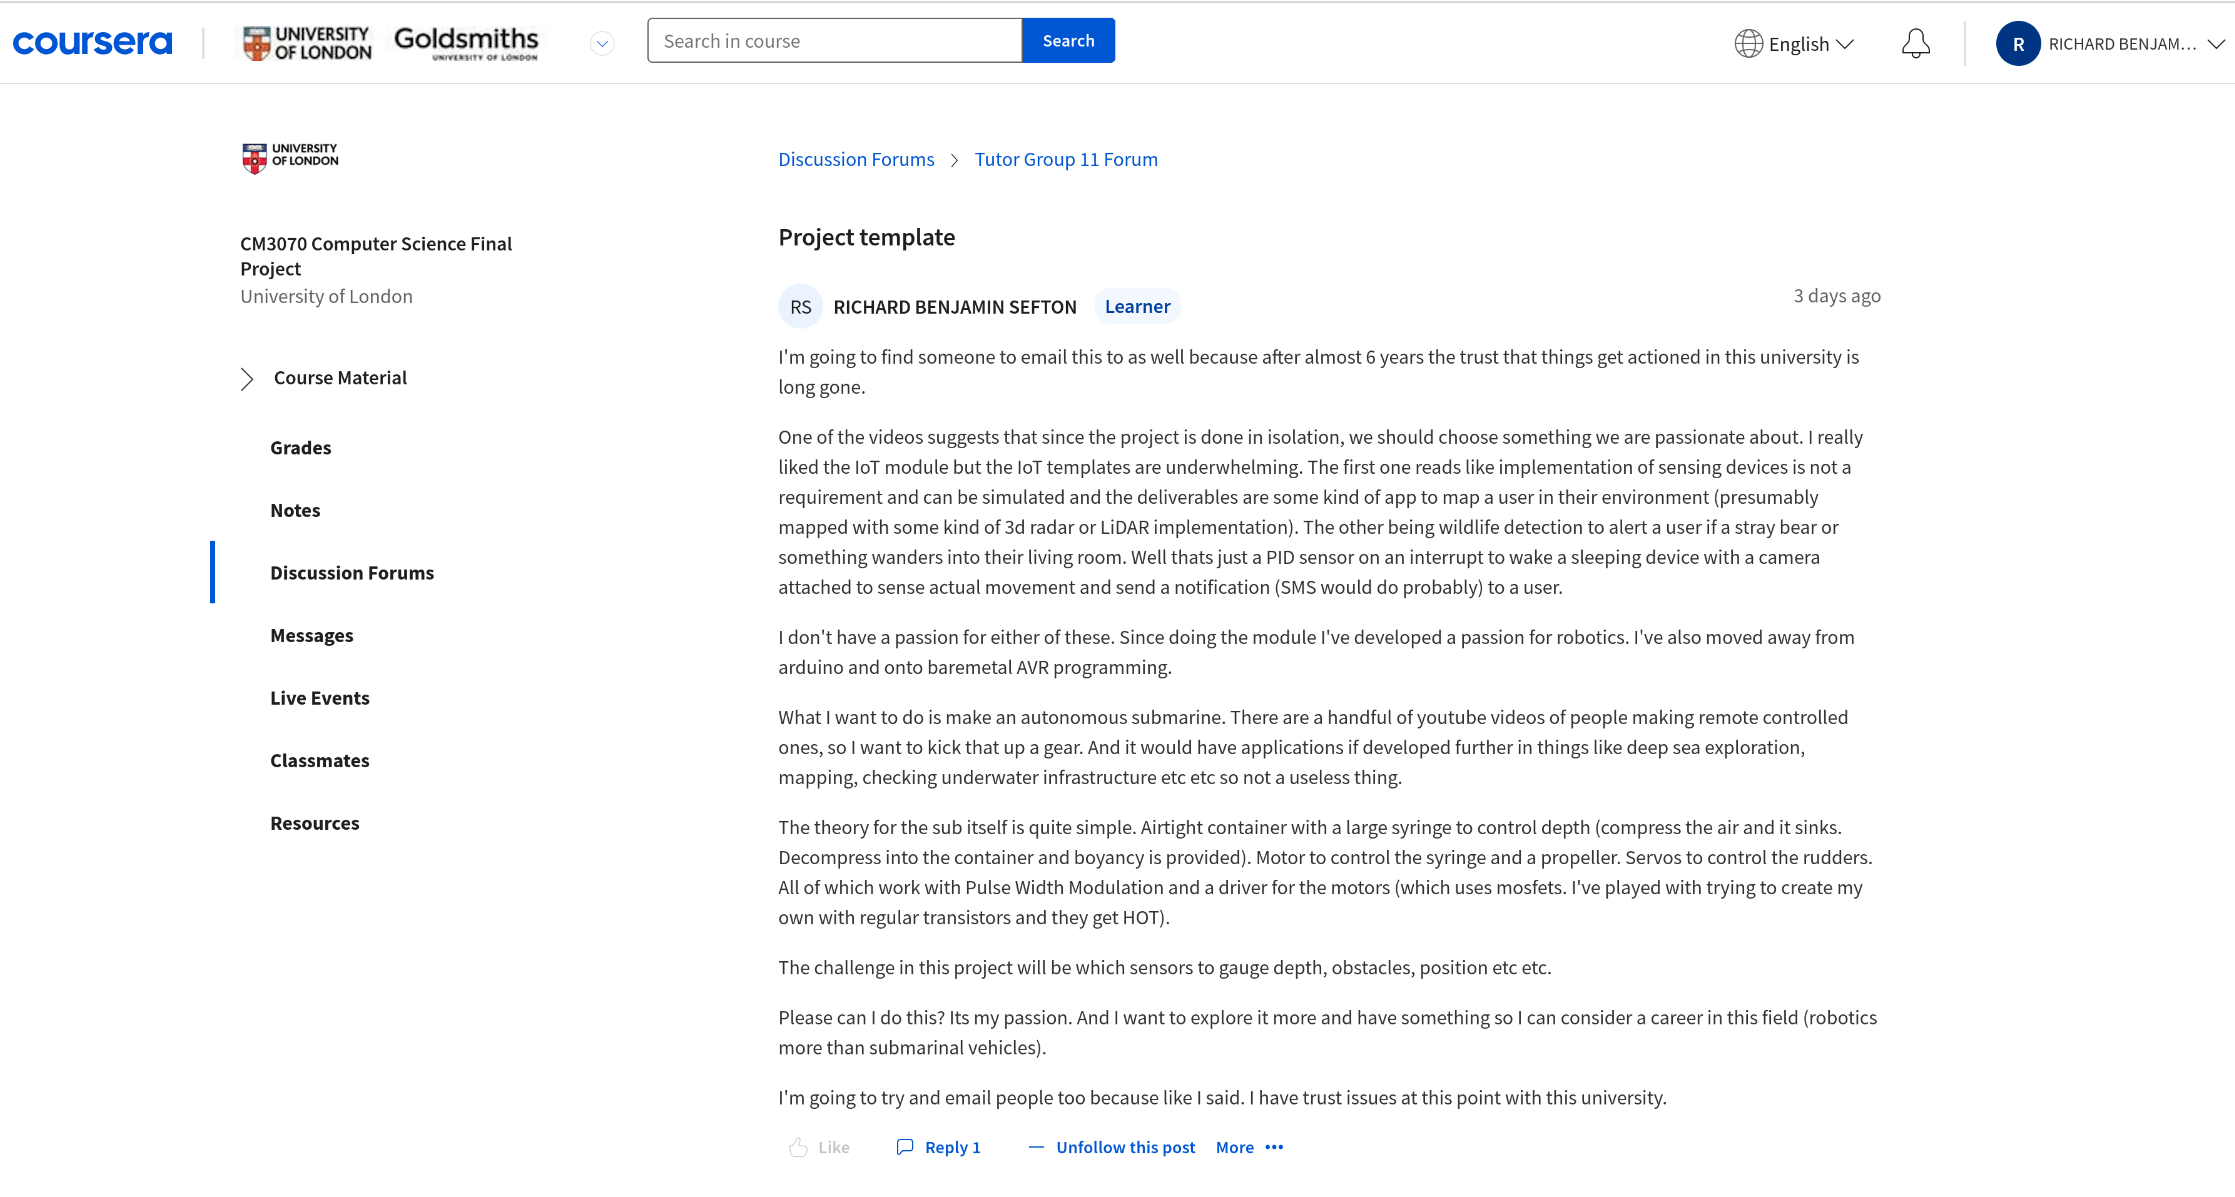
\includegraphics[scale=0.15]{assets/FinalProject_permission_1.png}
	\end{center}
	\begin{center}
		\label{picture:permission_2}
		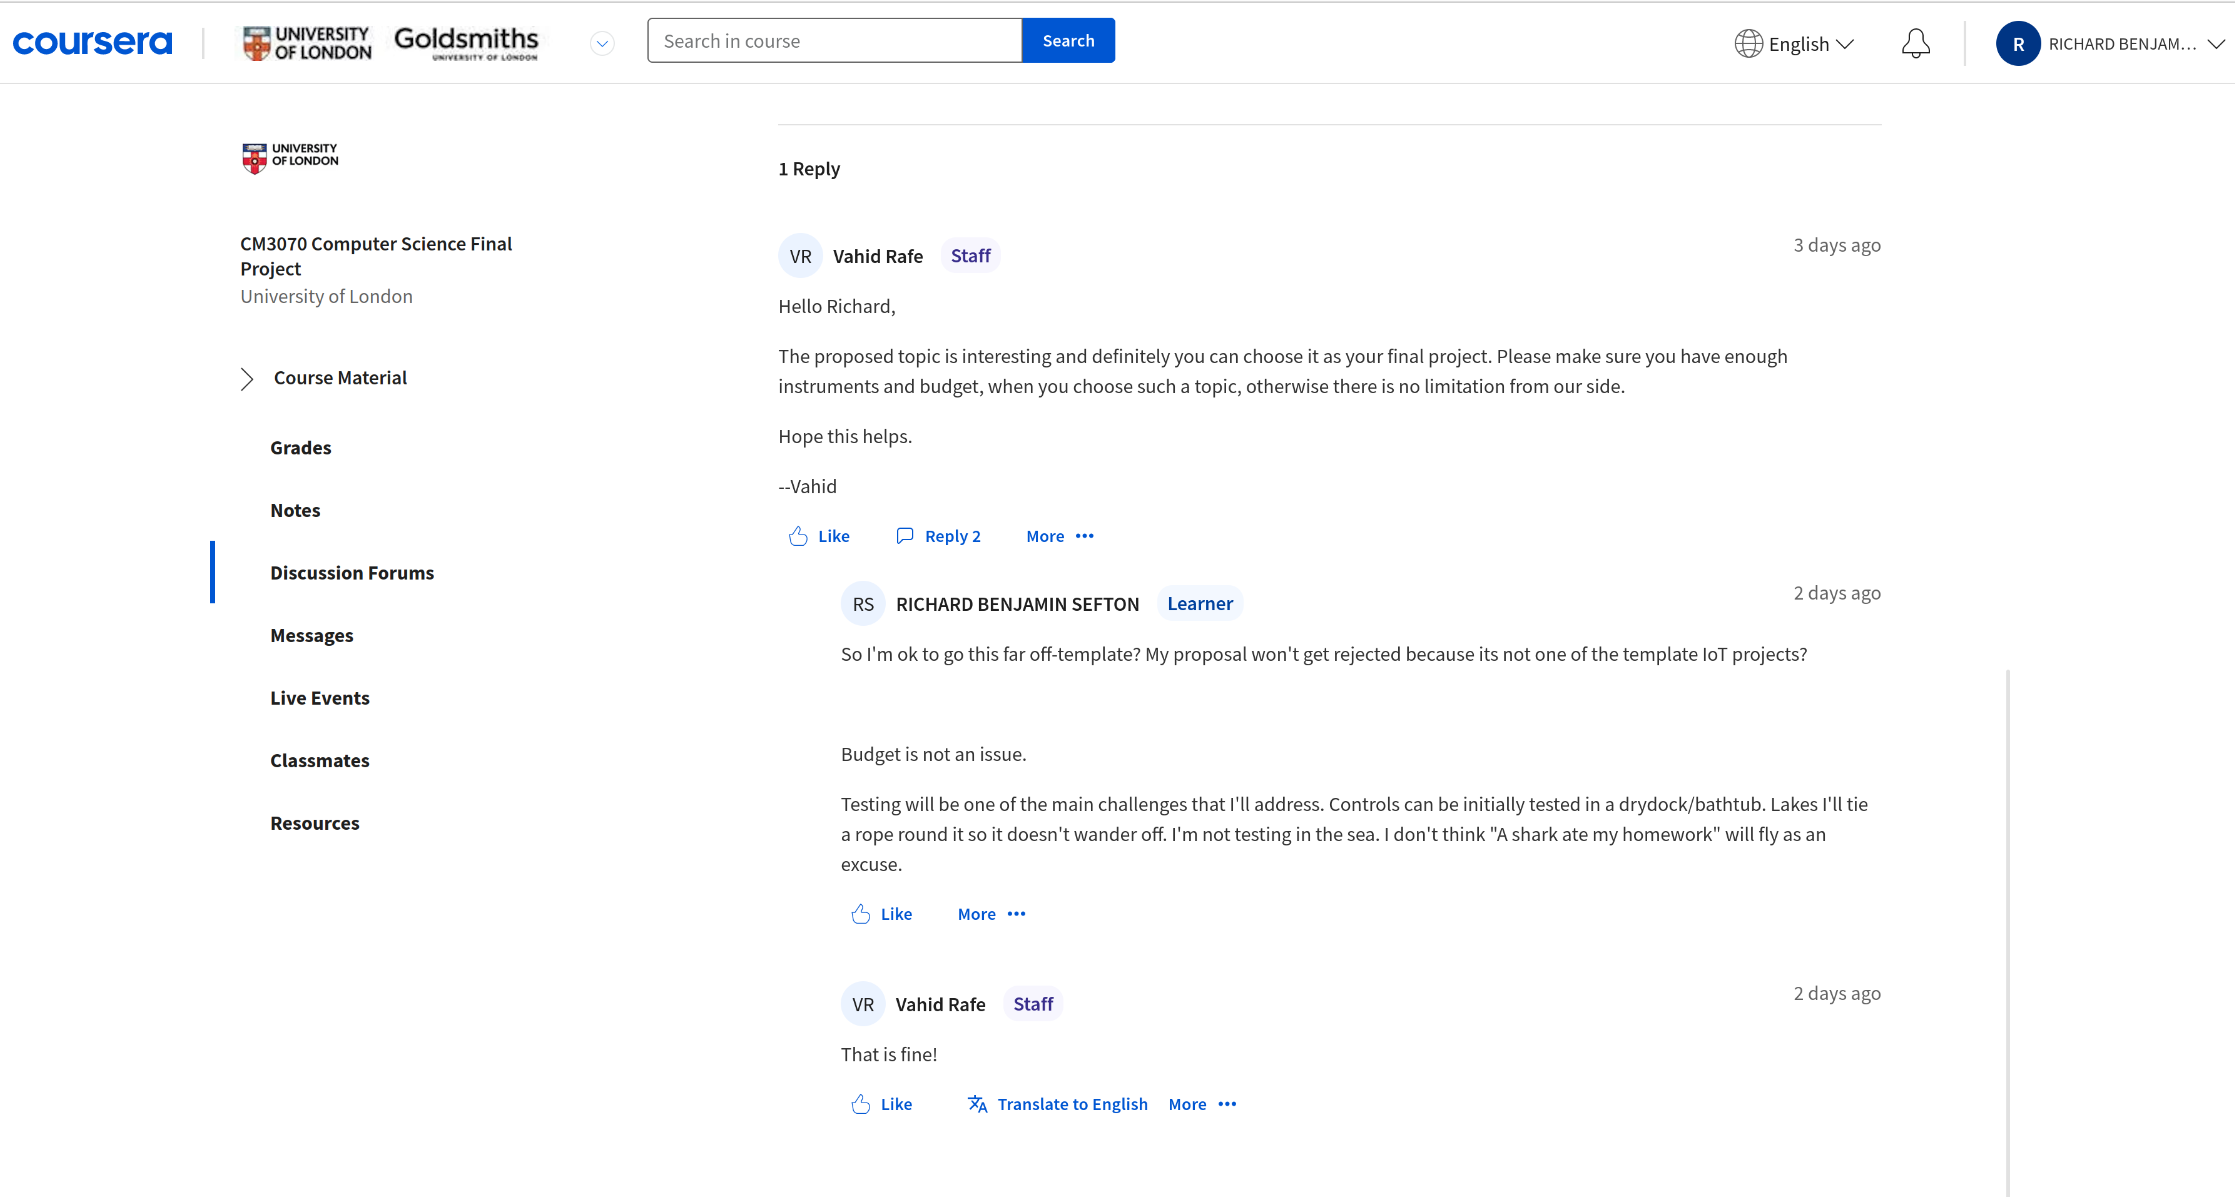
\includegraphics[scale=0.15]{assets/FinalProject_permission_2.png}
	\end{center}
	
	\chapter{Project Plan}\label{appendix:project_plan}
	\begin{center}
		\label{picture:gaant1}
		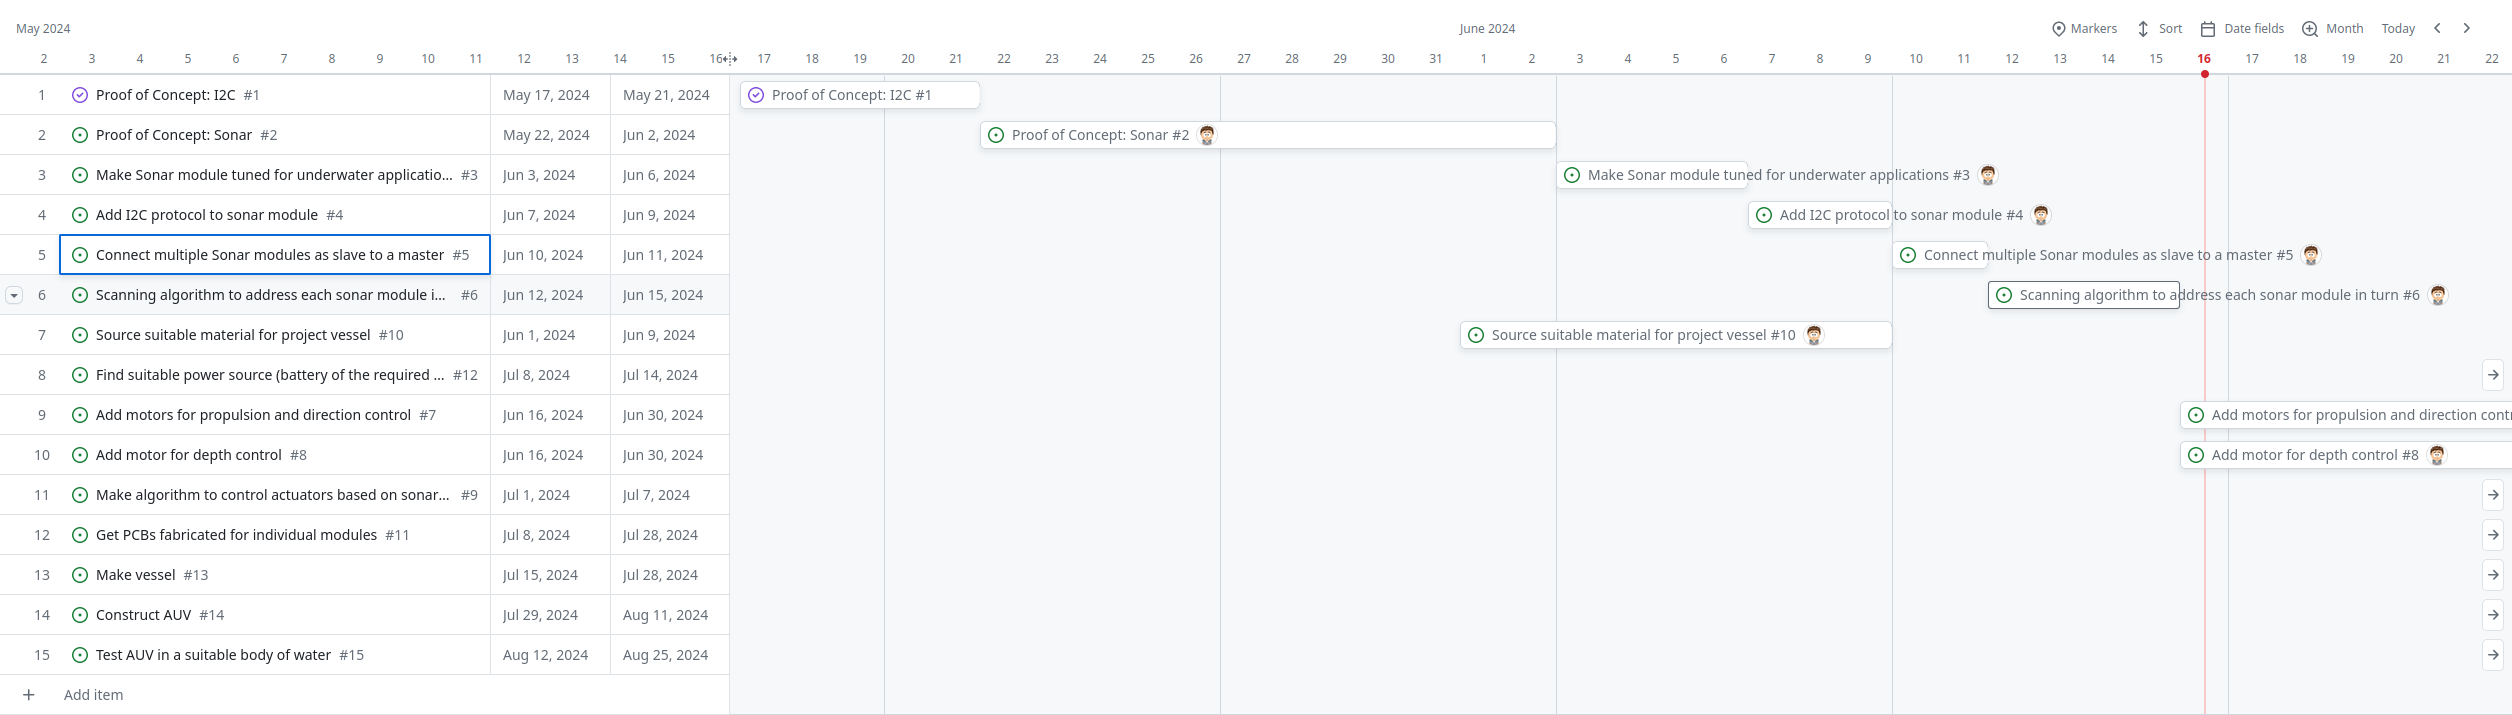
\includegraphics[scale=0.15]{assets/gannt_start-june22.png}
	\end{center}
	\begin{center}
		\label{picture:gaant2}
		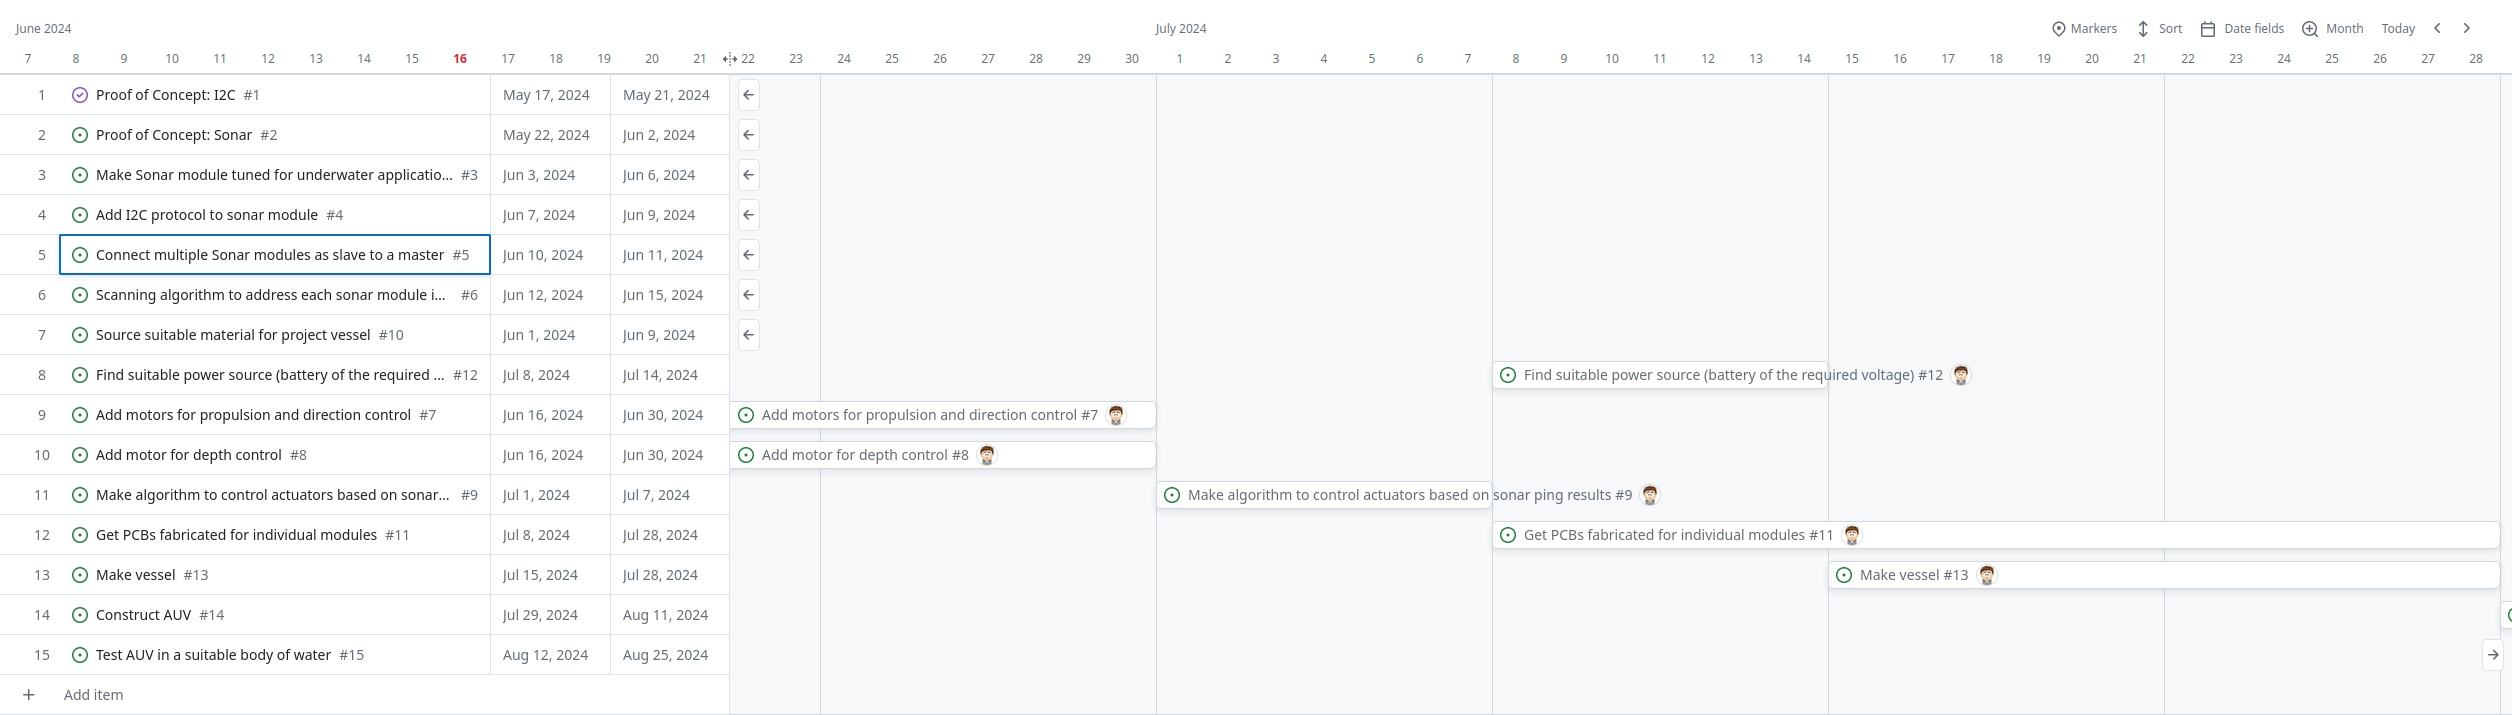
\includegraphics[scale=0.15]{assets/gaant_june22-july28.png}
	\end{center}
	\begin{center}
		\label{picture:gaant3}
		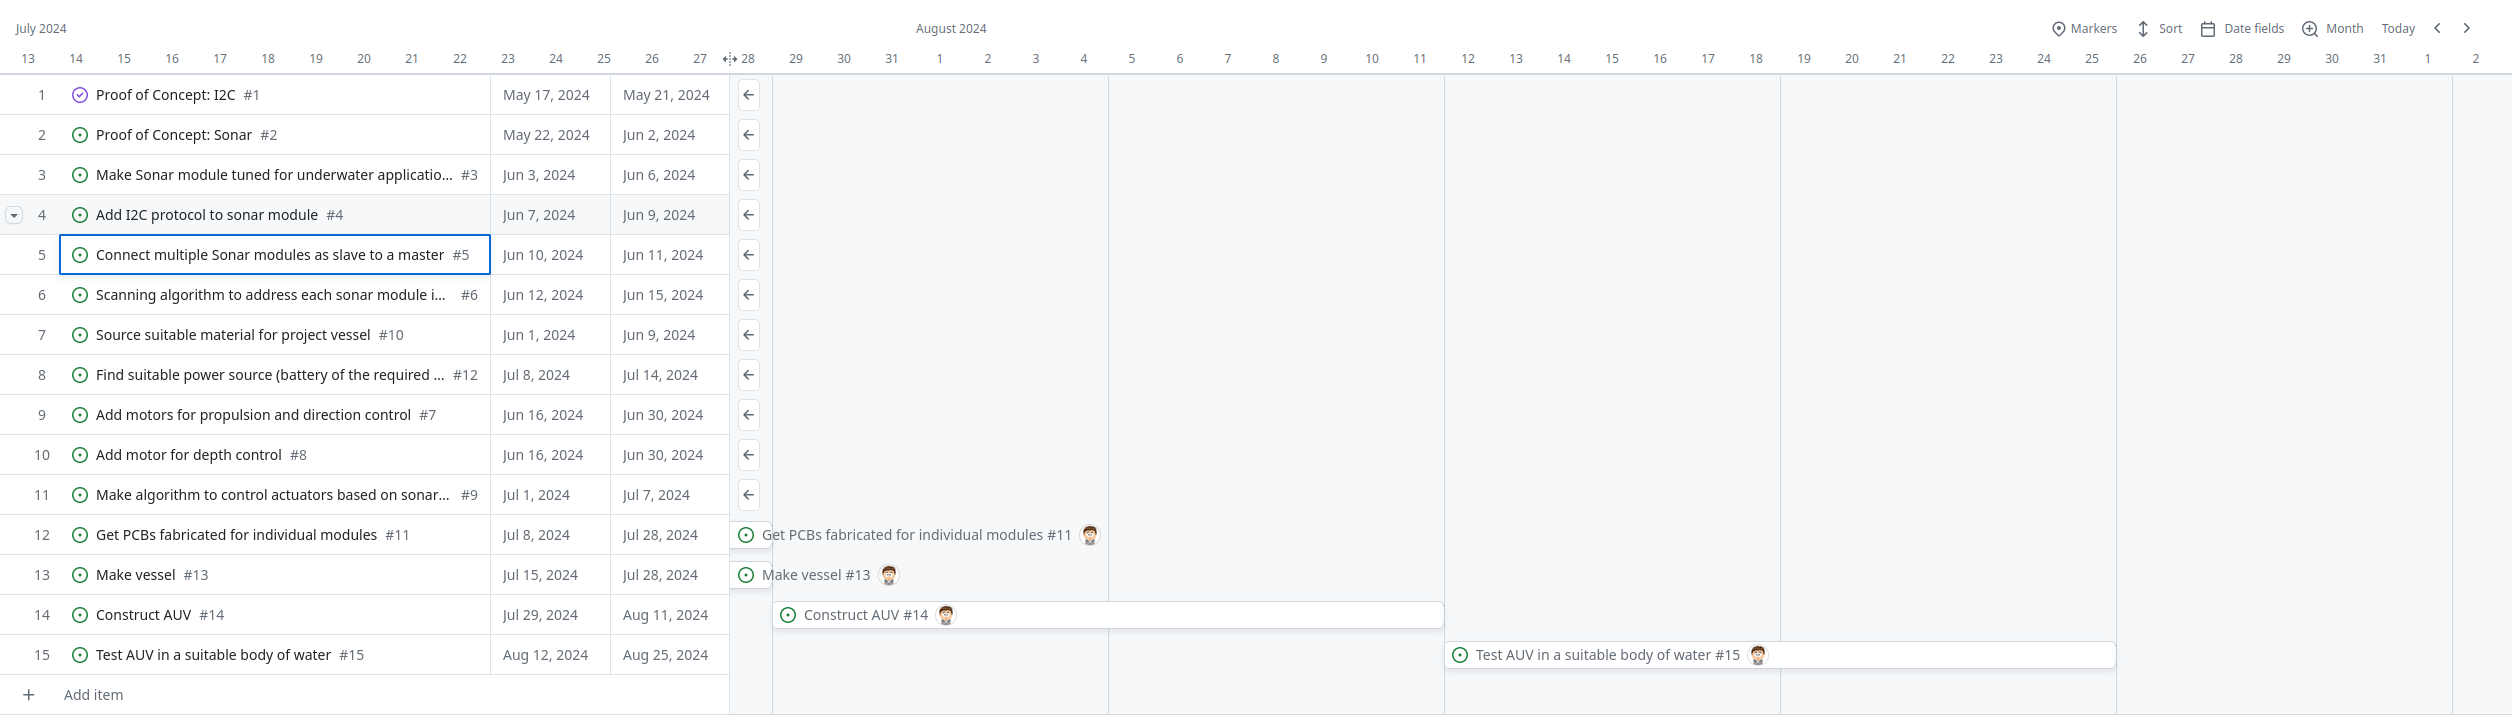
\includegraphics[scale=0.15]{assets/gaant_july28-sept2.png}
	\end{center}
	\begin{center}
		\label{picture:backlog}
		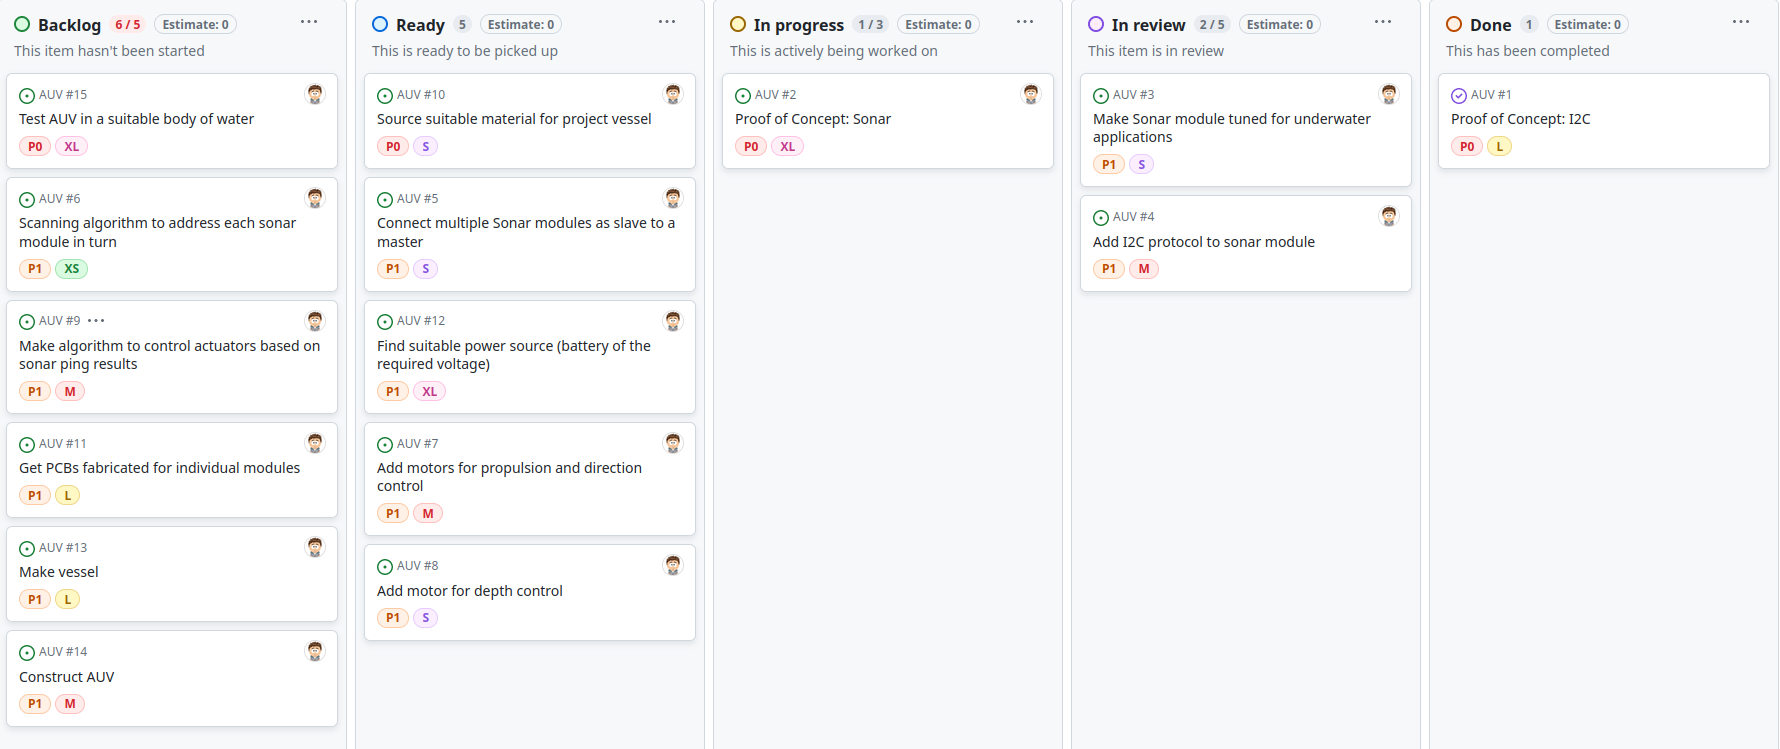
\includegraphics[scale=0.2]{assets/backlog.png}
	\end{center}
	\begin{center}
		\label{picture:priority}
		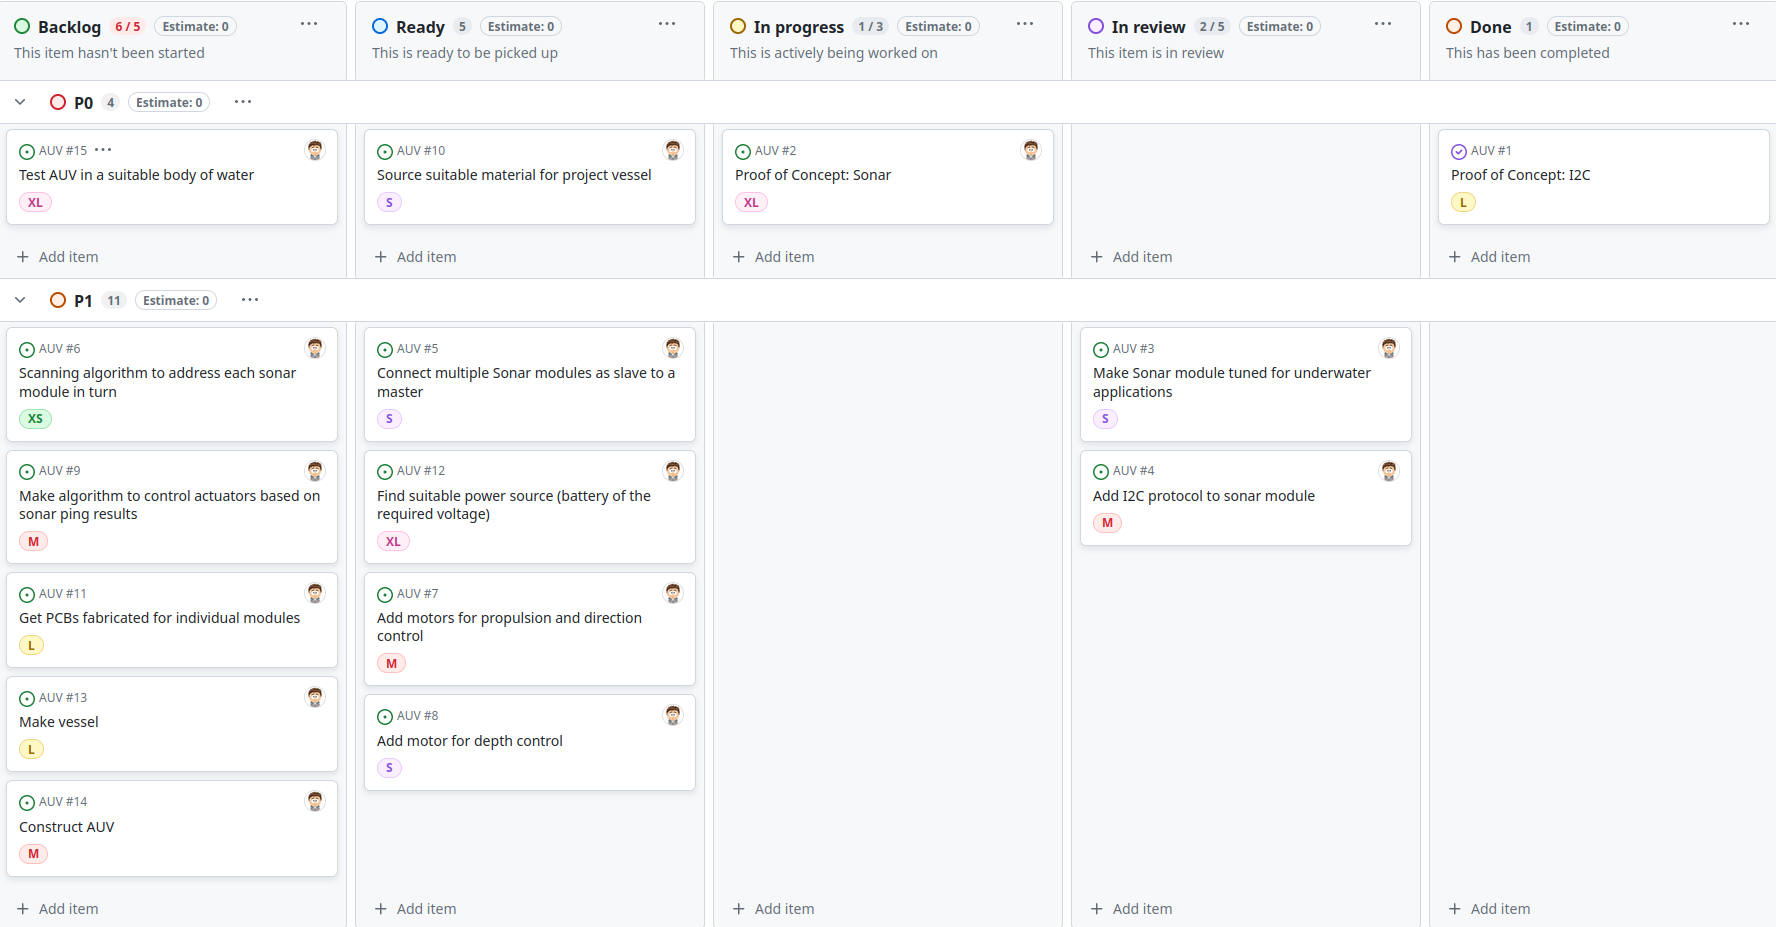
\includegraphics[scale=0.2]{assets/priority.png}
	\end{center}
	
	\chapter{VQFN Breakout}\label{appendix:vqfn_breakout}
	\begin{center}
		\label{picture:breakout1}
		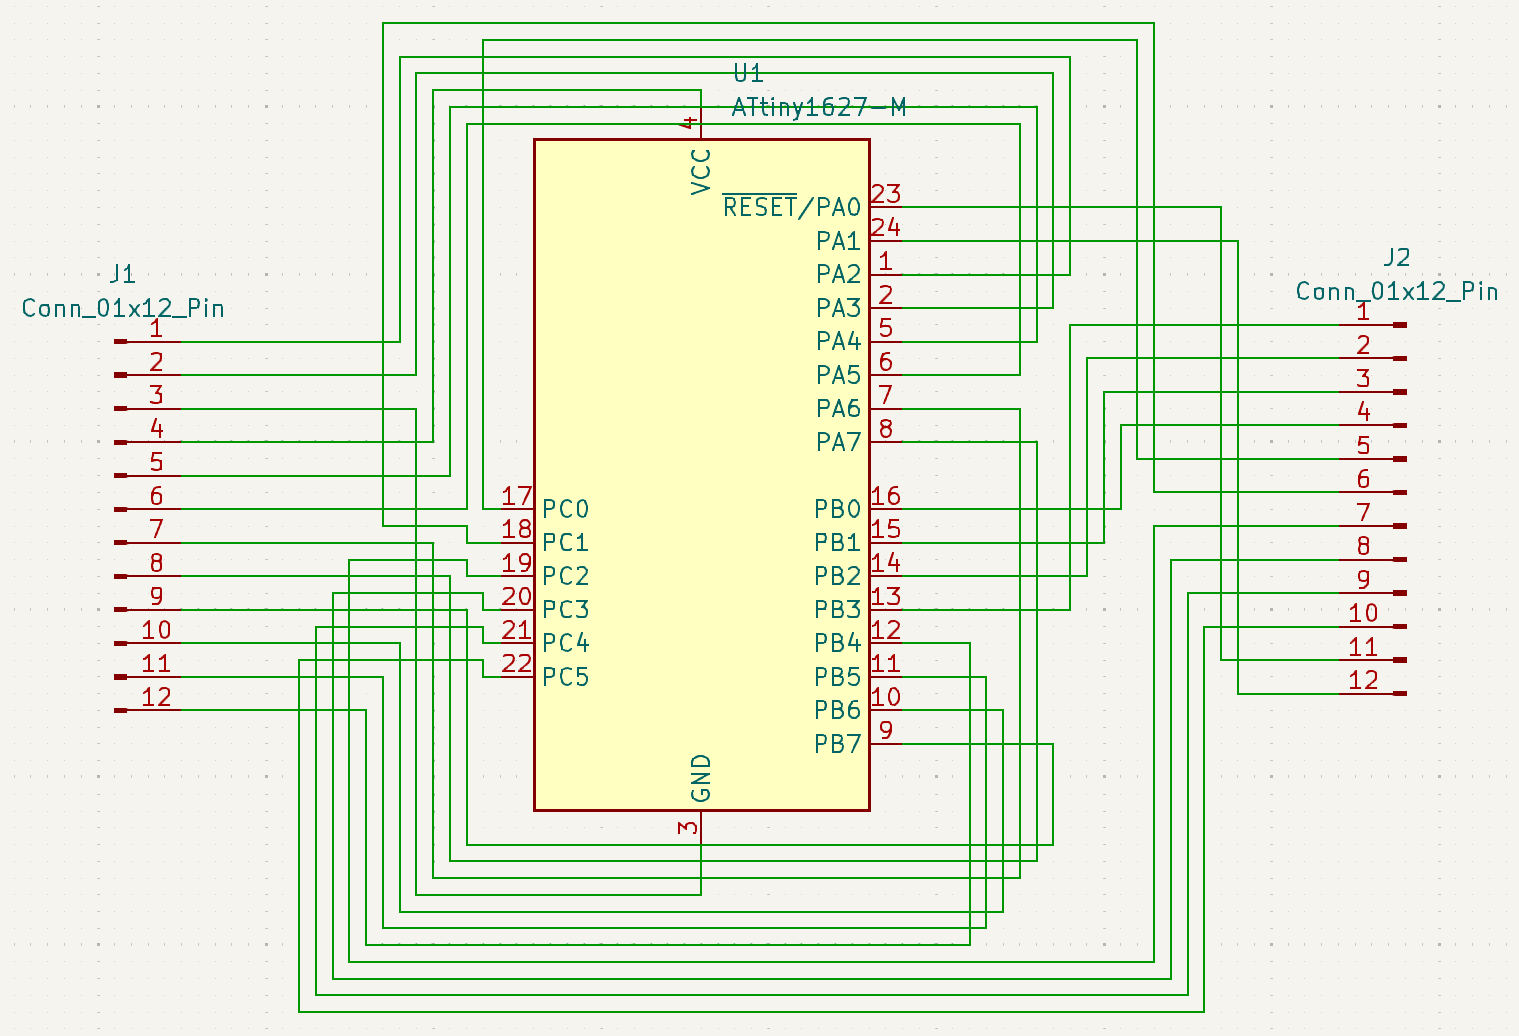
\includegraphics[scale=0.2]{assets/breakout_schematic.png}
	\end{center}
	\begin{center}
		\label{picture:breakout2}
		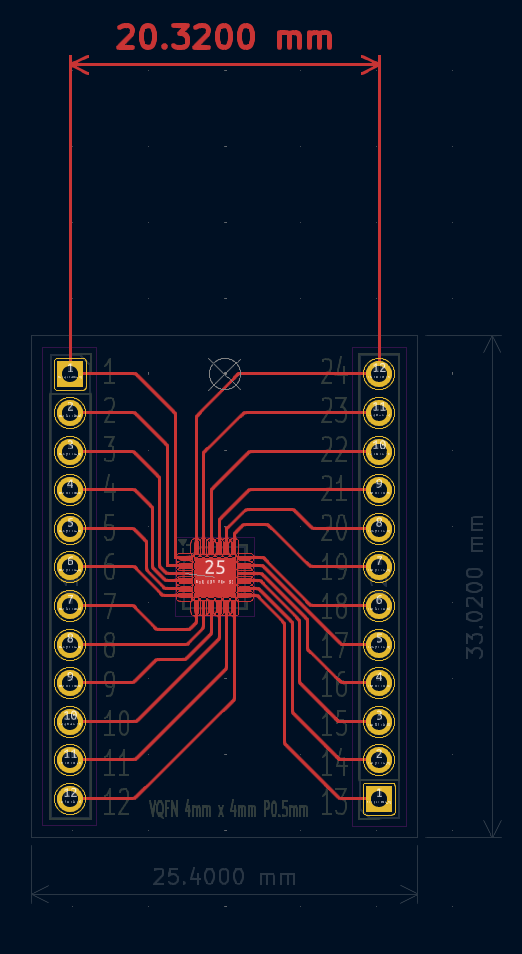
\includegraphics[scale=0.2]{assets/breakout_pcb_schema.png}
	\end{center}
		\begin{center}
		\label{picture:breakout3}
		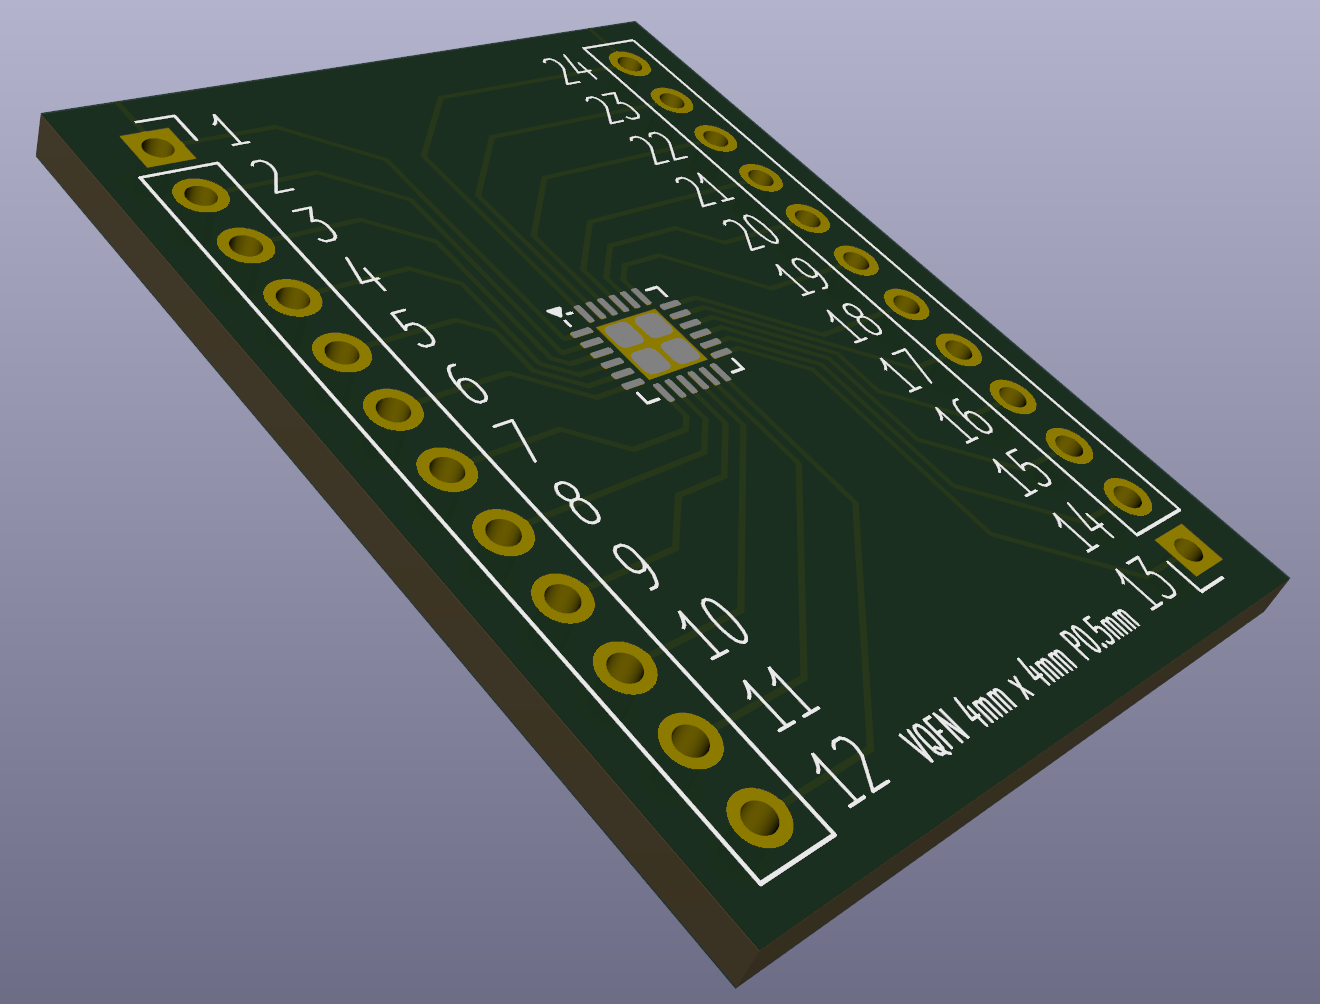
\includegraphics[scale=0.2]{assets/breakout_pcb_3d.png}
	\end{center}
	
	\chapter{AVR ATTiny 1627 Features}\label{appendix:attiny_features}
	\begin{itemize}
		\item Low Power
		\item 16\unit{\kilo\byte} programmable flash memory
		\item 256\unit{\byte} EEPROM
		\item Power on Reset
		\item Brown out Detection
		\item Configurable clock
		\item UPDI
		\item Idle, Standby and Power down sleep modes
		\item 3x 16 bit Timer Counters (TCA and 2 x TCB)
		\item PWM generation
		\item Real time Counter
		\item USART
		\item SPI
		\item TWI ($I^{2}C$)
		\item Analog to Digital conversion (ADC) with amplifier
		\item Watchdog Timer
		\item Interrupts on all GPIO pins
		\item 22 Programmable GPIO pins
	\end{itemize}
	
	\chapter*{Prototype Module Code}\label{appendix:prototype_module_code}
	\label{code:prototype_central_controller}
	\textbf{Central Controller code}
	\begin{lstlisting}
		#include <avr/io.h>
		#include <avr/interrupt.h>
		#include <util/delay.h>
		#include "TWI.h"
		
		#define MOTOR_DRIVER_ADDR 0x49
		#define SONAR_ADDR 0x08
		
		#define COM_STOP 0xFF
		#define COM_START 0xAA
		
		// LED For debugging
		#define RED PIN6_bm
		#define GREEN PIN5_bm
		#define BLUE PIN7_bm
		#define YELLOW (PIN6_bm | PIN5_bm)
		#define PURPLE (PIN6_bm | PIN7_bm)
		#define CYAN (PIN5_bm | PIN7_bm)
		#define WHITE (PIN6_bm | PIN5_bm | PIN7_bm)
		
		void MainClkCtrl(void);
		void SetupRTC(void);
		void SetupTCA(void);
		
		// For LED Debugging
		void SetupPins(void);
		void ChangeColour(uint8_t);
		
		volatile uint8_t distance = 0;
		volatile uint8_t sendMotorInstruction = 0;
		
		int main()
		{
			MainClkCtrl();
			
			// Allow Slaves to init first
			_delay_ms(2000);
			
			SetupRTC();
			SetupTCA();
			
			TWI_Master_Init();
			
			SetupPins();
			
			sei();
			
			while(1)
			{
				ChangeColour(GREEN);
			}
			
			return 0;
		}
		
		void MainClkCtrl(void) 
		{
			_PROTECTED_WRITE(CLKCTRL.MCLKCTRLA, CLKCTRL_CLKSEL_OSC20M_gc);
			_PROTECTED_WRITE(CLKCTRL.MCLKCTRLB, CLKCTRL_PDIV_6X_gc | CLKCTRL_PEN_bm);
			// F_CPU with this configuration will be 3.33MHz
		}
		
		void SetupRTC(void) 
		{
			RTC.CLKSEL |= RTC_CLKSEL_INT1K_gc;
			RTC.PER = 1024; //provides a 1 second interval timer
			// Clear any existing flags
			RTC.INTFLAGS |= RTC_OVF_bm;   
			// Enable the overflow interrupt
			RTC.INTCTRL |= RTC_OVF_bm;
			// Enable the RTC
			RTC.CTRLA |= RTC_RTCEN_bm;
		}
		
		void SetupTCA(void)
		{
			// Set up TCA to overflow at a desired interval
			TCA0.SINGLE.PER = 0xFFFF; // Maximum period
			// Enable TCA overflow interrupt
			TCA0.SINGLE.INTCTRL |= TCA_SINGLE_OVF_bm;
			// Set TCA to Normal mode
			TCA0.SINGLE.CTRLB |= TCA_SINGLE_WGMODE_NORMAL_gc;
			// Use the system clock and set prescaler
			TCA0.SINGLE.CTRLA |= TCA_SINGLE_CLKSEL_DIV1_gc;
		}
		
		void SetupPins(void)
		{
			PORTB.DIR |= RED | GREEN | BLUE;
		}
		
		void ChangeColour(uint8_t c)
		{
			PORTB.OUTSET = RED | GREEN | BLUE;
			PORTB.OUTCLR = c;
		}
		
		ISR(RTC_CNT_vect)
		{
			// Clear the interrupt flag
			RTC.INTFLAGS = RTC_OVF_bm; 
			
			ChangeColour(RED);
			
			// Start TWI operation
			distance = 0; //reset the distance
			TWI_Master_Start(SONAR_ADDR, 0x01); //Start TWI to sonar module 
			distance = TWI_Master_Read_NACK(); //Get the distance
			TWI_Master_Start((uint8_t)MOTOR_DRIVER_ADDR, 0x00); //Start TWI to Motor
			if (distance < 55)
			{
				TWI_Master_Write(COM_STOP); //Send motor a stop command
			}
			else
			{
				TWI_Master_Write(COM_START); //Send motor a start command. 
			}
			TWI_Master_Stop();
			
			ChangeColour(PURPLE);
		}
	\end{lstlisting}
	\newpage
	\label{code:ultrasonic}
	\textbf{Ultrasonic Module code}
	\begin{lstlisting}
		#include <avr/io.h>
		#include <avr/interrupt.h>
		#include <util/delay.h>
		
		#include "TWI.h"
		
		#define ADDR 0x08
		
		#define COM_SCAN 0xFF
		
		void MainClkCtrl(void);
		void SetupPins(void);
		void SetupRTC(void);
		void I2C_RX_Callback(uint8_t);
		uint8_t I2C_TX_Callback(void);
		
		uint8_t waitingForEcho = 0;
		uint16_t startTime = 0.0;
		uint16_t endTime = 0;
		float distance = 0.0;
		float speedOfSound = 0.0343; // cm per microsecond
		float ticks = 0.0;
		
		int main()
		{
			MainClkCtrl();
			SetupPins();
			SetupRTC();
			
			TWI_Slave_Init(ADDR, I2C_RX_Callback, I2C_TX_Callback);
			
			sei();
			
			while(1)
			{
				// Main loop does nothing, waiting for interrupts
			}
			
			return 0;
		}
		
		void MainClkCtrl(void) 
		{
			_PROTECTED_WRITE(CLKCTRL.MCLKCTRLA, CLKCTRL_CLKSEL_OSC20M_gc);
			_PROTECTED_WRITE(CLKCTRL.MCLKCTRLB, CLKCTRL_PDIV_6X_gc | CLKCTRL_PEN_bm);
			// F_CPU with this configuration will be 3.33MHz
		}
		
		void SetupPins(void)
		{
			// Trigger
			PORTA.DIR |= PIN2_bm;
			
			// Echo
			PORTA.DIR &= ~(PIN3_bm);
			//    PORTA.PIN3CTRL = PORT_ISC_FALLING_gc;
		}
		
		void SetupRTC(void) {
			RTC.CLKSEL = RTC_CLKSEL_INT32K_gc;
			// Wait for synchronization
			while (RTC.STATUS & RTC_CTRLABUSY_bm);
			RTC.PER = 0xFFFF; //Maximum period
			// Enable the RTC, run in standby mode, no prescaler
			RTC.CTRLA = RTC_RUNSTDBY_bm | RTC_PRESCALER_DIV1_gc | RTC_RTCEN_bm;
		}
		
		void I2C_RX_Callback(uint8_t com)
		{
			// We're not actually using this. Just need the function for the SlaveInit function
		}
		
		uint8_t I2C_TX_Callback(void)
		{
			// Set trigger pin to high
			PORTA.OUTSET = PIN2_bm;
			_delay_us(10);  // Wait at least 10us
			PORTA.OUTCLR = PIN2_bm;  // Disable trigger
			startTime = RTC.CNT;
			
			// Wait for echo pin to go high
			while (!(PORTA.IN & PIN3_bm));
			
			// Wait for echo pin to go low
			while (PORTA.IN & PIN3_bm);
			
			// Read RTC counter value
			endTime = RTC.CNT;
			
			// Calculate distance
			ticks = (float)(endTime - startTime) * 30.5176; // Convert to microseconds
			distance = (ticks * speedOfSound) / 2;
			
			// Return the calculated distance as a byte
			return (uint8_t)distance;
		}
	\end{lstlisting}
	\newpage
	\label{code:motor}
	\textbf{Motor Controller code}
	\begin{lstlisting}
		#define F_CPU 3333333UL
		#include <avr/io.h>
		#include <util/delay.h>
		#include "TWI.h"
		
		void MainClkCtrl(void);
		void SetupPins(void);
		void digitalWrite(uint8_t, uint8_t);
		void I2C_RX_Callback(uint8_t);
		uint8_t  I2C_TX_Callback(void);
		
		#define HIGH 0x01
		#define LOW 0x00
		
		#define STOP 0xFF
		#define FORWARD 0xAA
		#define BACKWARD 0x02
		
		#define ADDR 0x49
		
		volatile uint8_t state = FORWARD;
		volatile uint8_t step = 0x00;
		
		
		void stepperMotorStep(uint8_t step);
		
		int main()
		{
			MainClkCtrl();
			SetupPins();
			TWI_Slave_Init(ADDR, I2C_RX_Callback, I2C_TX_Callback);
			
			while(1)
			{
				if (state != STOP)
				{
					stepperMotorStep(step);
					
					if(state == FORWARD)
					{
						step++;
					}
					else
					{
						step--;
					}
					
					if(step > 0x07)
					{
						step = 0x00;
					}
					
					if(step < 0x00)
					{
						step = 0x07;
					}
					
					_delay_us(750); // Adjust delay as needed    
				}
			}
			
			return 0;
		}
		
		void MainClkCtrl(void) 
		{
			_PROTECTED_WRITE(CLKCTRL.MCLKCTRLA, CLKCTRL_CLKSEL_OSC20M_gc);
			_PROTECTED_WRITE(CLKCTRL.MCLKCTRLB, CLKCTRL_PDIV_6X_gc | CLKCTRL_PEN_bm); // Prescaler of 6
			// F_CPU with this configuration will be 3.33MHz
		}
		
		void SetupPins()
		{
			PORTA.DIR |= PIN4_bm | PIN5_bm | PIN6_bm | PIN7_bm;
		}
		
		void digitalWrite(uint8_t pin, uint8_t value)
		{
			if (value == LOW)
			{
				PORTA.OUTCLR = pin;
			}
			else
			{
				PORTA.OUTSET = pin;
			}
		}
		
		void stepperMotorStep(uint8_t step)
		{
			//This is basically from the datasheet http://eeshop.unl.edu/pdf/Stepper+Driver.pdf
			//Made the digitalWrite function to keep it inline. 
			switch (step)
			{
				case 0:
				digitalWrite(PIN4_bm, LOW);
				digitalWrite(PIN5_bm, LOW);
				digitalWrite(PIN6_bm, LOW);
				digitalWrite(PIN7_bm, HIGH);
				break;
				case 1:
				digitalWrite(PIN4_bm, LOW);
				digitalWrite(PIN5_bm, LOW);
				digitalWrite(PIN6_bm, HIGH);
				digitalWrite(PIN7_bm, HIGH);
				break;
				case 2:
				digitalWrite(PIN4_bm, LOW);
				digitalWrite(PIN5_bm, LOW);
				digitalWrite(PIN6_bm, HIGH);
				digitalWrite(PIN7_bm, LOW);
				break;
				case 3:
				digitalWrite(PIN4_bm, LOW);
				digitalWrite(PIN5_bm, HIGH);
				digitalWrite(PIN6_bm, HIGH);
				digitalWrite(PIN7_bm, LOW);
				break;
				case 4:
				digitalWrite(PIN4_bm, LOW);
				digitalWrite(PIN5_bm, HIGH);
				digitalWrite(PIN6_bm, LOW);
				digitalWrite(PIN7_bm, LOW);
				break;
				case 5:
				digitalWrite(PIN4_bm, HIGH);
				digitalWrite(PIN5_bm, HIGH);
				digitalWrite(PIN6_bm, LOW);
				digitalWrite(PIN7_bm, LOW);
				break;
				case 6:
				digitalWrite(PIN4_bm, HIGH);
				digitalWrite(PIN5_bm, LOW);
				digitalWrite(PIN6_bm, LOW);
				digitalWrite(PIN7_bm, LOW);
				break;
				case 7:
				digitalWrite(PIN4_bm, HIGH);
				digitalWrite(PIN5_bm, LOW);
				digitalWrite(PIN6_bm, LOW);
				digitalWrite(PIN7_bm, HIGH);
				break;
			}
		}
		
		void I2C_RX_Callback(uint8_t com)
		{
			if (com == STOP) 
			{
				state = STOP;
			}
			else if (com == FORWARD)
			{
				state = FORWARD;
			}
			else if (com == BACKWARD)
			{
				state = BACKWARD;
			}
			else
			{
				state = STOP;
			}
		}
		
		uint8_t I2C_TX_Callback(void)
		{
			//Not used, but needed for SlaveInit
		}
	\end{lstlisting}
	
	\chapter{TWI Library Code}\label{appendix:twi_library}
	\label{code:twi_h}
	\textbf{TWI.h}
	\begin{lstlisting}
		#ifndef TWI_H
		#define TWI_H
		
		#include <avr/io.h>
		#include <avr/interrupt.h>
		#include <stddef.h> 
		
		/*
		* Macros used to help calculate the BAUD rate for the TWI/I2C Protocol. 
		* 
		* The formulas can be found on the datasheet.
		*/
		//only if not defined. 
		#ifndef F_CPU
		#define F_CPU 3333333UL
		#endif
		#define TWI_FREQ 100000UL //1MHz
		#define TWI_BAUD(F_SCL, T_RISE) ((((F_CPU / (F_SCL)) - 10) / 2) - (T_RISE / 2))
		
		/*
		* Callback functions for the Slave initialisation of the protocol. This will be 
		* called by the ISR for Slave received requests so the code that implements this 
		* library can provide functionality without having to customise the library itself,
		* and call helper functions outside the scope of the library. 
		*/
		typedef void (*I2C_ReceiveCallback)(uint8_t data);
		typedef uint8_t (*I2C_TransmitCallback)(void);
		
		// TWI/I2C Master functions
		/**
		* This function initialises the TWI/I2C Protocol on a device designated as the master
		* where it will be able to specify and send requests to the connected slave devices. 
		*/
		void TWI_Master_Init(void);
		
		/**
		* This function will try to force the TWI protocol back into its starting state. 
		* This is to stop an issue where repeated requests are crashing the device. 
		*/
		void TWI_Master_Reset(void);
		
		/**
		* This function will put the protocol in a state where it is able to either read or 
		* write data. It will target a slave, and specify if its a read or write operation. 
		* 
		* Read         0x01
		* Write        0x00
		* 
		* @param address       The Slave address to be contacted
		* @param read          The mode of operation (Read, Write)
		*/
		void TWI_Master_Start(uint8_t address, uint8_t read);
		
		/**
		* This function will perform the Write operation. The function will write data to the
		* MDATA buffer which should transfer to the Slave. 
		* 
		* At the moment, this library will only really send a single uint8_t (one byte) of 
		* data. 
		* 
		* @param data          Data to be sent. 
		*/
		void TWI_Master_Write(uint8_t data);
		
		/**
		* This function will read from the MDATA buffer for data sent from the Slave on Read
		* operations. The device will then send an ACK (0) to confirm it is ready for more 
		* data. 
		* 
		* @return              Data received from the Slave
		*/
		uint8_t TWI_Master_Read_ACK(void);
		
		/**
		* This function will read from the MDATA buffer for data sent from the Slave on Read
		* operations. The device will then send an NACK (1) to tell the Slave it can't accept 
		* more data. 
		* 
		* @return              Data received from the Slave
		*/
		uint8_t TWI_Master_Read_NACK(void);
		
		/**
		* This function issues a stop command to the protocol to cease transmissions. 
		* 
		* This should then put the bus in an IDLE state. 
		*/
		void TWI_Master_Stop(void);
		
		// I2C Slave functions
		/**
		* This function will initialise the I2C Protocol on Slave devices. It will set the 
		* address to the SADDR buffer, and set the callback functions so they can be called
		* by the ISR when an address is confirmed and the mode of operation is identified. 
		* 
		* In Read operations the data should be returned by the TX callback function so the ISR
		* can pick it up and continue. In the current state we can't just leave this function hanging. 
		* It MUST return a value that will be sent so we can't rely on interrupts to populate a value.
		* 
		* In Write operations the data from the Master will be sent to the RX callback function.  
		* @param address       The address of the Slave device. Requests from the Master will work on this device. 
		* @param               The RX Callback function
		* @param               The TX Callback function
		*/
		void TWI_Slave_Init(uint8_t address, I2C_ReceiveCallback, I2C_TransmitCallback);
		
		/**
		* This function will send data to the Master device. It will write data to the SDATA
		* buffer which will be transmitted to the Master. 
		* 
		* @param data          The data to be sent
		*/
		void TWI_Slave_Write(uint8_t data);
		
		/**
		* This function will read data from the Master device. It will get the data sent by 
		* reading from the SDATA buffer. 
		* 
		* @return              The received data
		*/
		uint8_t TWI_Slave_Read(void);
		
		/**
		* Same as above but explicitly sends ACK
		* @return 
		*/
		uint8_t TWI_Slave_Read_ACK(void);
		
		/**
		* Same as above but explicitly sends NACK and Transaction Complete command. 
		* @return 
		*/
		uint8_t TWI_Slave_Read_NACK(void);
		
		#endif // TWI_H
	\end{lstlisting}
	\newpage
	\label{code:twi_c}
	\textbf{TWI.c}
	\begin{lstlisting}
		#include "TWI.h"
		
		/* Initialize TWI/I2C master - TWI is AVR version that supports I2C since I2C is a 
		* protocol made by Phillips and supported by many MCUs.
		* 
		* This library is developed using the datasheet and the Make: AVR Programming book
		* with some reference to libraries such as https://github.com/technoblogy/tiny-i2c
		* 
		* Finding code examples online is a challenge and they need to be adapted because
		* the ATTiny1627 is not widely used as say anything from the ATMega line. Typically
		* users of the Tiny series use chips such as the ATTiny45 or similar that comes in a 
		* DIP (breadboard friendly) packaging. 
		* 
		* Also alot of the existing libraries are focused towards Arduino which I'm trying 
		* to move away from.
		*/
		
		void TWI_Master_Init(void) 
		{
			/* Set the TWI baud rate
			* This calculation should for the ATTiny1627 on standard speed come to ~12
			* but because the way C handles float conversion to uint8, the fractional is dropped 
			* and the result rounded down. So we're adding one at the end to combat this.
			*/ 
			TWI0.MBAUD = (uint8_t)TWI_BAUD(TWI_FREQ, 0) + 1; // Adding 1 as it is rounding down
			
			/* Enable TWI master and Smart Mode
			* Smart mode will automatically raise the DIF, RIF and WIF interrupt flags when
			* reading from and or writing to the MDATA, SDATA and MADDR buffers. This takes
			* a fair bit of the work out of our hands, but may raise some issues when we come 
			* to ending the Read operation as the Master should send a NACK to RXACK with a 
			* stop condition to end the operation. 
			*/
			TWI0.MCTRLA |= TWI_ENABLE_bm | TWI_SMEN_bm;
			
			/**
			* Writing to the Flush bit on the MCTRLB register will flush any errors or bus busy states
			* try to force the protocol into IDLE. Since in this implementation we only have 
			* one Master, this should work but I've never writen a protocol from scratch before
			* so I guess we'll find out..
			*/
			TWI0.MCTRLB |= TWI_FLUSH_bm; // Flush TWI data
			
			// Explicitly set the bus state to IDLE.
			TWI0.MSTATUS = TWI_BUSSTATE_IDLE_gc;
			
			// Enable the Master Write Interrupt and Master Read Interrupt
			TWI0.MCTRLA |= TWI_WIEN_bm | TWI_RIEN_bm;
			
			/**
			* Because some implementations of this library may not need Interrupts (Motor 
			* Controller is a key suspect here), we should enable Interrupts so code in this
			* library will still work. 
			*/
			sei();
		}
		
		void TWI_Master_Reset(void)
		{
			// Disable TWI by writing a zero to the enable bit
			TWI0.MCTRLA &= ~TWI_ENABLE_bm;
			
			// Clear status registers to reset the state
			TWI0.MSTATUS |= TWI_BUSERR_bm | TWI_ARBLOST_bm | TWI_RXACK_bm | TWI_COLL_bm | TWI_BUSSTATE_IDLE_gc;
			//    TWI0.MCTRLB |= TWI_FLUSH_bm; // Flush TWI
			
			// Re-enable TWI
			TWI0.MCTRLA |= TWI_ENABLE_bm;
		}
		
		void TWI_Master_Start(uint8_t address, uint8_t read)
		{
			TWI0.MADDR = (address << 1) | read;
			//Wait for the address transmission to complete. When the address is confirmed 
			//by the slave, the WIF or RIF flags will be raised. 
			while (!(TWI0.MSTATUS & (TWI_RIF_bm | TWI_WIF_bm)));
		}
		
		void TWI_Master_Write(uint8_t data) 
		{
			TWI0.MDATA = data;
			
			//Wait for the WIF to become high. Writing data will set it low (Smart mode),
			//When the Slave receives it will be set back to high. 
			while (!(TWI0.MSTATUS & TWI_WIF_bm));
			
			// Check for arbitration lost or bus error
			if (TWI0.MSTATUS & (TWI_ARBLOST_bm | TWI_BUSERR_bm)) {
				// Handle error
				TWI0.MCTRLB = TWI_FLUSH_bm;
				TWI0.MSTATUS = TWI_BUSSTATE_IDLE_gc;
			}
		}
		
		uint8_t TWI_Master_Read_ACK(void) 
		{
			//    //Temporarily Disable SM
			//    TWI0.MCTRLA &= ~TWI_SMEN_bm;
			//Prime the MCTRLB with the ACK bit
			TWI0.MCTRLB = TWI_ACKACT_ACK_gc;
			
			//Wait till the device has received data
			while (!(TWI0.MSTATUS & TWI_RIF_bm));
			
			//return the data from the buffer. Smart mode should then send the ACK bit and 
			//clear the relevant flags.
			return TWI0.MDATA;
		}
		
		uint8_t TWI_Master_Read_NACK(void) 
		{
			//Temporarily Disable SM
			//    TWI0.MCTRLA &= ~TWI_SMEN_bm;
			
			//Prime the MCTRLB with the NACK bit
			TWI0.MCTRLB = TWI_ACKACT_NACK_gc;
			
			//Wait till the device has received the data
			while (!(TWI0.MSTATUS & TWI_RIF_bm));
			
			TWI0.MCTRLB |= TWI_MCMD_STOP_gc;
			//Return the data from the buffer. Smart mode should then send the NACK bit 
			//and clear the relevant flags
			uint8_t data = TWI0.MDATA;
			
			//    TWI0.MCTRLB |= TWI_MCMD_STOP_gc;
			
			//Renable SM
			//    TWI0.MCTRLA |= TWI_SMEN_bm;
			
			//    return TWI0.MDATA;
			return data;
		}
		
		/**
		* DO NOT CALL ARBITRARILY. THIS COULD PUT THE BUS IN AN ERROR STATE.
		*/
		void TWI_Master_Stop(void) {
			TWI0.MCTRLB = TWI_MCMD_STOP_gc;
			//    TWI0.MSTATUS = TWI_BUSSTATE_IDLE_gc; 
		}
		
		// Global variable to store the receive callback function
		static I2C_ReceiveCallback receive_callback = NULL;
		static I2C_TransmitCallback transmit_callback = NULL;
		
		void TWI_Slave_Init(uint8_t address, I2C_ReceiveCallback rx, I2C_TransmitCallback tx) 
		{
			//Assign the RX and TX callback functions so they can be accessed by this script (raise their scope). 
			receive_callback = rx;
			transmit_callback = tx;
			
			// Set the slave address. << 1 as the first bit is for enabling broadcast mode on 0x00
			TWI0.SADDR = address << 1;
			
			// Enable TWI slave and various interrupts. Also Smart Mode. 
			TWI0.SCTRLA |= TWI_ENABLE_bm | TWI_SMEN_bm | TWI_DIEN_bm | TWI_APIEN_bm | TWI_PIEN_bm;
			
			sei();
		}
		
		void TWI_Slave_Write(uint8_t data) {
			//Write the data to the buffer to send to the Master. This should clear the DIF interrupt. 
			TWI0.SDATA = data;
			
			//When the Master has received the data the DIF interrupt should be high again. 
			while (!(TWI0.SSTATUS & TWI_DIF_bm));
			
			if (TWI0.SSTATUS & TWI_RXACK_bm)
			{
				//Master send dobby an NACK. END TRANSMISSION
				TWI0.SCTRLB |= TWI_SCMD_COMPTRANS_gc;
			}
			
			// Clear the DIF
			//    TWI0.SSTATUS |= TWI_DIF_bm;
			
		}
		
		uint8_t TWI_Slave_Read(void) {
			//Wait for the data to be ready. 
			while (!(TWI0.SSTATUS & TWI_DIF_bm));
			
			//Read the data from the buffer
			uint8_t data = TWI0.SDATA;
			
			// Clear the data interrupt flag
			//THIS SHOULDNT BE REQUIRED BECAUSE SMART MODE. 
			//    TWI0.SSTATUS |= TWI_DIF_bm;
			
			
			return data;
		}
		
		uint8_t TWI_Slave_Read_ACK(void) {
			// Wait for the data to be ready
			while (!(TWI0.SSTATUS & TWI_DIF_bm));
			
			// Read the data from the buffer
			uint8_t data = TWI0.SDATA;
			
			// Send ACK after receiving data
			TWI0.SCTRLB = TWI_ACKACT_ACK_gc;
			
			return data;
		}
		
		uint8_t TWI_Slave_Read_NACK(void) {
			// Wait for the data to be ready
			while (!(TWI0.SSTATUS & TWI_DIF_bm));
			
			//     Send NACK after receiving data
			TWI0.SCTRLB = TWI_ACKACT_NACK_gc;
			
			return TWI0.SDATA;
		}
		
		/**
		* Interrupt Service Routines
		* 
		* This is how the Slave will begin responding to the requests. 
		* 
		* First it will check the address. AP is an address match. Clearing the flag will 
		* trigger the Master to begin its operation. 
		* 
		* DIF is raised when data is received or Master is ready to receive. the DIR register bit
		* will identify which mode of operation it is. 
		*/
		ISR(TWI0_TWIS_vect) 
		{
			// Check if Address/Stop interrupt
			//    if (TWI0.SSTATUS & TWI_APIF_bm) {
				//        // Clear the interrupt flag
				//        TWI0.SSTATUS |= TWI_APIF_bm;
				//        // Check if the address match
				//        if (TWI0.SSTATUS & TWI_AP_bm) {
					//            // Clear the address match flag
					//            TWI0.SSTATUS |= TWI_AP_bm;
					//        }
				//    }
			// Check if Address/Stop interrupt
			if (TWI0.SSTATUS & TWI_APIF_bm)
			{
				// Clear the interrupt flag
				TWI0.SSTATUS = TWI_APIF_bm;
				
				// Check if the address match
				if (TWI0.SSTATUS & TWI_AP_bm)
				{
					// Clear the address match flag
					TWI0.SSTATUS = TWI_AP_bm;
					TWI0.SCTRLB = TWI_SCMD_RESPONSE_gc;
				}
				//        else
				//        {
					//            // If not an address match, it must be a stop condition
					//            TWI0.SCTRLB = TWI_SCMD_COMPTRANS_gc;
					//        }
			}
			
			// Check if Data interrupt
			if (TWI0.SSTATUS & TWI_DIF_bm) {
				// Check if data was requested (read operation)
				if (TWI0.SSTATUS & TWI_DIR_bm) {
					//Get the data from the callback function passed in in initialisation. 
					//Should handle cases where this is NULL. but eh. Not for this this implementation. 
					uint8_t data_to_send = transmit_callback();
					TWI_Slave_Write(data_to_send);  // Example data
				} else {
					//Read the received data. 
					uint8_t received_data = TWI_Slave_Read_NACK();
					//Send the data to the callback function
					receive_callback(received_data);
				}
				
				TWI0.SSTATUS |= TWI_DIF_bm;
			}
		}
	\end{lstlisting}
	
	\chapter{Sonar Schematics}\label{appendix:sonar_schematics}
	
	\textbf{Transmitter}
	\begin{center}
		\label{picture:sonar_schema1}
		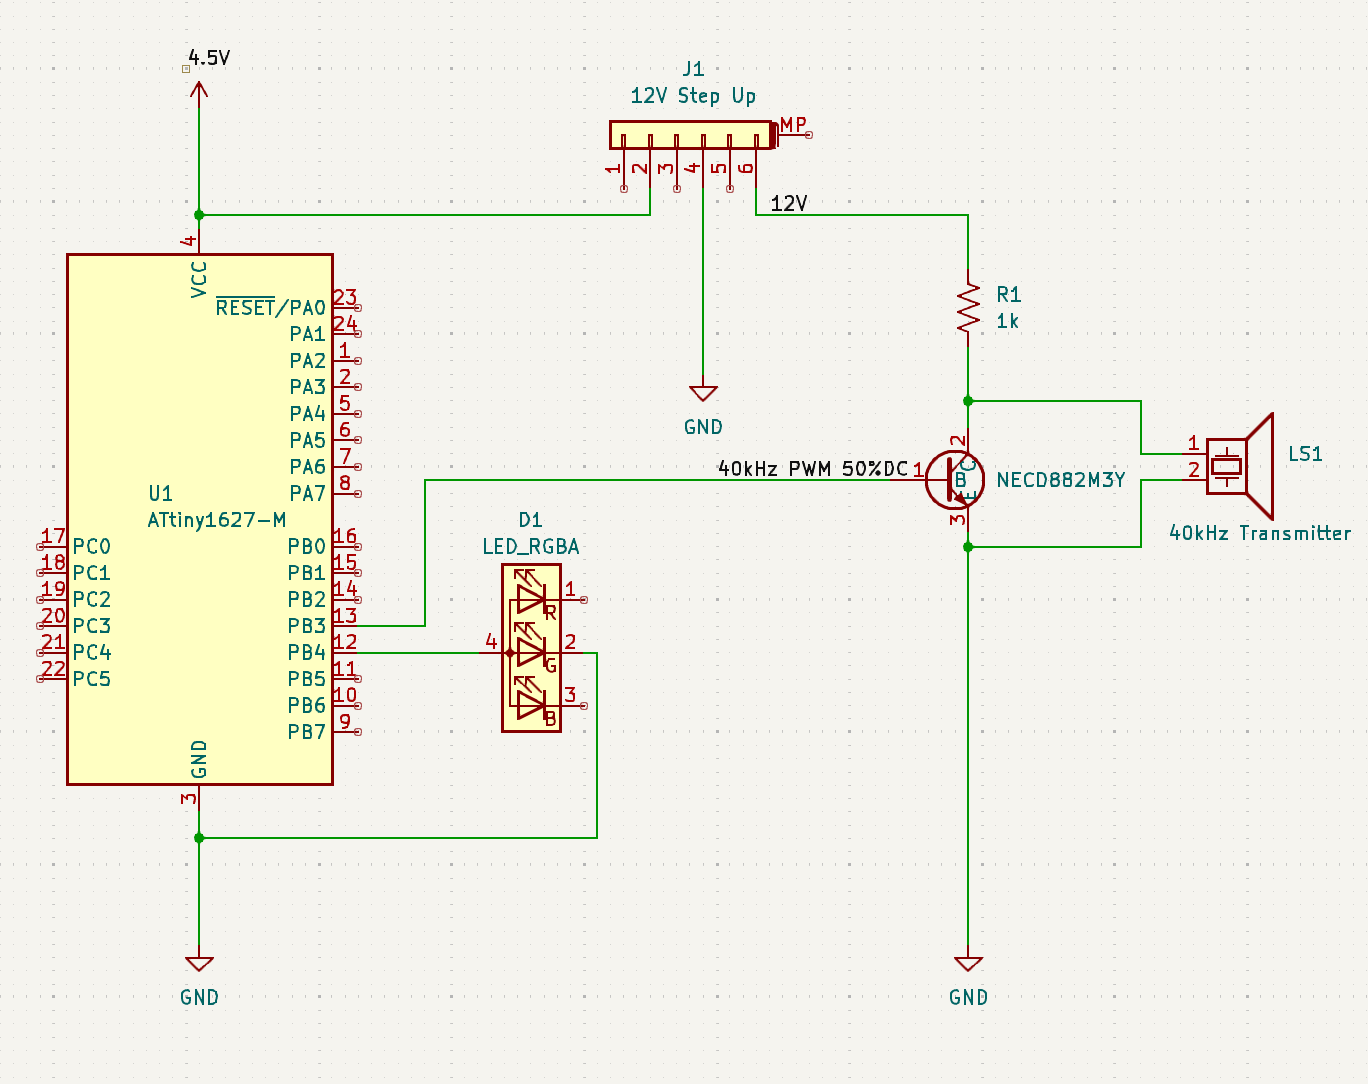
\includegraphics[scale=0.3]{assets/sonar_transmitter.png}
	\end{center}
	\newpage
	\textbf{Receiver}
	\begin{center}
		\label{picture:sonar_schema2}
		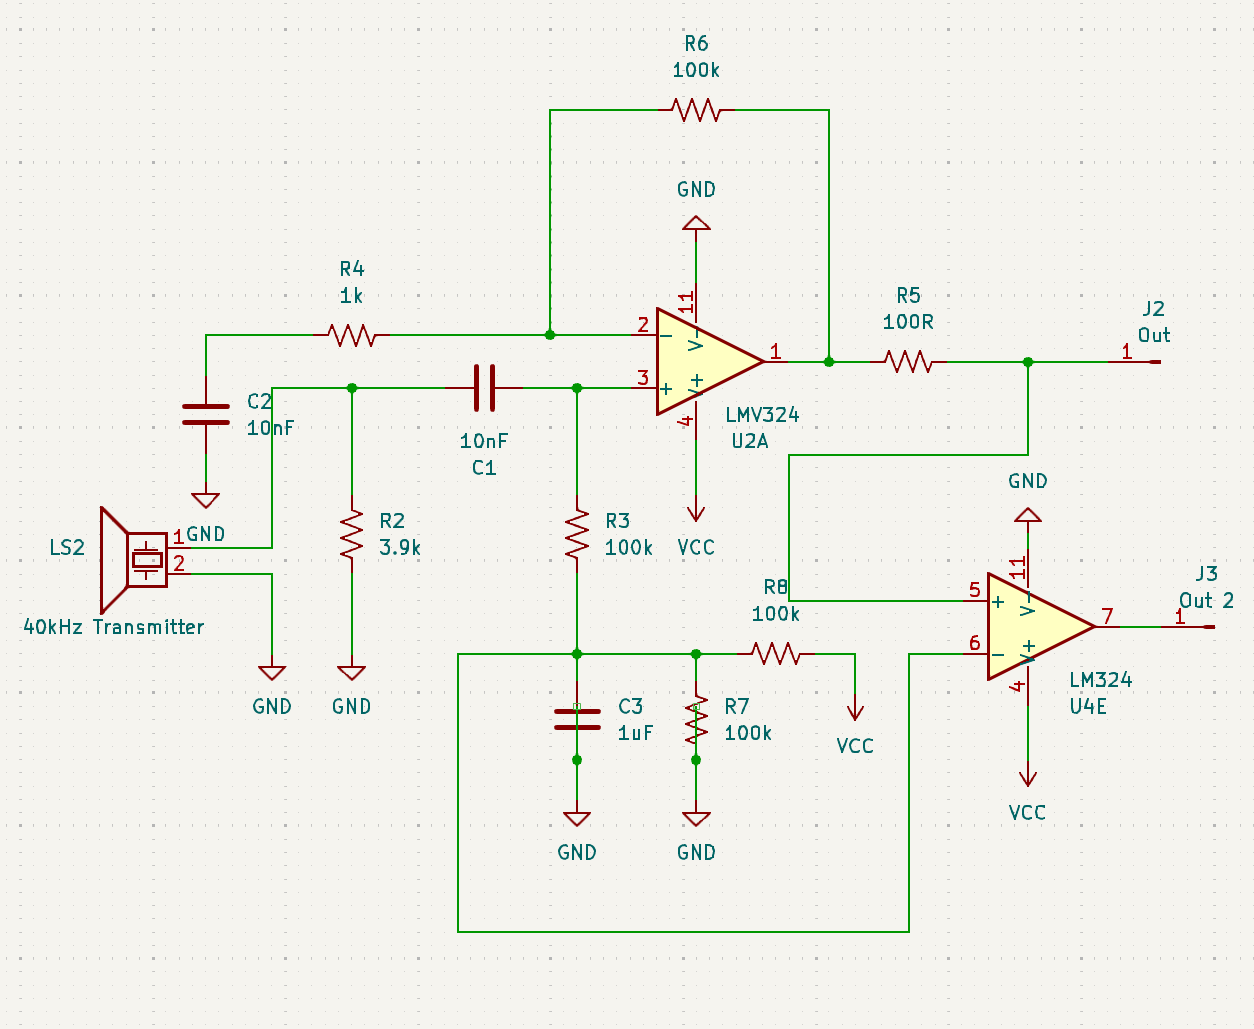
\includegraphics[scale=0.3]{assets/sonar_receiver.png}
	\end{center}
	
	\chapter{Depth Controller}\label{appendix:depth_controller}
	\begin{lstlisting}
		/**
		* This is the depth controller for the submarine. 
		* 
		* This is a stepper motor connected to a convertor of my own design to convert
		* linear to rotary force. Its basically a screw connected to a large nut with a housing for the syringe 
		* plunger. 
		* 
		* So basically this controller needs to control the stepper motor in two directions (forward
		* and reverse), and also make sure the motor does not turn beyond a certain point in either direction. 
		* 
		* Basically we need a way to track the position of the nut. 
		*/
		
		//Lets get the basics out the way. 
		#define F_CPU 3333333UL
		#include <avr/io.h>
		#include <util/delay.h>
		#include <avr/interrupt.h>
		
		void MainClkCtrl(void);
		
		/**
		* Need a way to track the position. I'm thinking an array. As the motor turns, 
		* every second or so we can either increment or decrement the array based on direction. 
		* 
		* If the array is at the start of end, we can't progress. It would be neat. As long 
		* as theres no reset of the device. 
		* 
		* Option 2 would be a wire and a contact plate so we know where at the start or the
		* end of the rail.
		* 
		* I think both. So in cases where the device has no power at non-start or stop position its 
		* reference isn't completely lost. 
		* 
		* To traverse the array we'll have a Timer Counter that will increment the index after a 
		* set period
		*/
		volatile uint8_t pos[30];
		void PosSetup(void);
		void BufferSetup(void);
		void RTCSetup(void);
		void PosDec(void);
		void PosInc(void);
		
		/*
		* Motor driver. We can steal this from the midterm prototype. which in itself was 
		* stolen from some forum describing how to use stepper motors with arduino. I think it 
		* was the original stepper motor datasheet but this was a while ago. - I just read its
		* comments. It was from the datasheet
		* 
		* So we need a digital write function
		* 
		* We also need to rejig the pins its using. 
		* 
		* And have a setup function to setup the pins 
		*/
		void MotorSetup(void);
		void StepperMotorStep(int8_t);
		void digitalWrite(uint8_t, uint8_t);
		#define HIGH 0x01
		#define LOW 0x00
		//Contols the step
		volatile int8_t step = 1; //needs to be signed so it can slip into negative values
		
		/**
		* Need a way to control the direction. We'll use some constants and a direction variable
		* 
		* There are 3 possible directions. UP, DOWN and NONE
		*/
		#define UP 0
		#define NONE 1
		#define DOWN 2
		volatile uint8_t dir = 2;
		
		int main(void)
		{
			MainClkCtrl();
			PosSetup(); 
			BufferSetup();
			
			MotorSetup();
			
			sei();
			
			while(1)
			{
				//1 is the marker number. If the element is 1, it means the device thinks the 
				//nut is in that position. so we won't go any further. 
				if (dir == UP && pos[29] != 1)
				{
					StepperMotorStep(step);
					step--;
				}
				else if (dir == DOWN && pos[0] != 1)
				{
					StepperMotorStep(step);
					step++;
				}
				
				//Keep the step in bounds
				if(step > 0x07)
				{
					step = 0x00;
				}
				
				if(step < 0x00)
				{
					step = 0x07;
				}
				
				_delay_us(750); //controls the speed. Adjust as needed. 
			}
			
			return 0;
		}
		
		/**
		* I think I've mentioned this in a previous part. This MCU has a default clock speed
		* of 3.33MHz. (20MHz with a default prescaler of 6). These settings are fine so we're 
		* just going to make it explicit. 
		*/
		void MainClkCtrl(void) 
		{
			_PROTECTED_WRITE(CLKCTRL.MCLKCTRLA, CLKCTRL_CLKSEL_OSC20M_gc | CLKCTRL_CLKOUT_bm);
			_PROTECTED_WRITE(CLKCTRL.MCLKCTRLB, CLKCTRL_PDIV_6X_gc | CLKCTRL_PEN_bm);
		}
		
		/*
		* Basically we're going to 0 the array and make the midpoint (512) 1. 
		* It will sort itself out in travel with the buffer
		*/
		void PosSetup(void)
		{
			for (int i = 0; i < 30; i++)
			{
				pos[i] = 0;
			}
			pos[15] = 1;
		}
		
		/**
		Buffer setup is the setup function for the start/stop plate we can use to reset the array to
		* make sure we don't go out of bounds.
		*/
		void BufferSetup(void)
		{
			//Pins to avoid are 15(PB1) and 16(PB0) as these are SDA and SCL respectively. 
			//also 23 (PA0) is the UPDI pin. 
			
			//Going to use 6(PA5), 7(PA6). These need to be inputs to detect voltage
			//    PORTA.DIR &= ~(PIN5_bm | PIN6_bm);
			PORTA.DIR &= ~(PIN5_bm);
			PORTA.DIR &= ~(PIN6_bm);
			//    PORTA.IN |= PIN5_bm | PIN6_bm;
			
			//Gonna need the interrupts on these
			//Because these pins are floating they need a pullup. 
			PORTA.PIN5CTRL |= PORT_PULLUPEN_bm | PORT_ISC_RISING_gc;
			PORTA.PIN6CTRL |= PORT_PULLUPEN_bm | PORT_ISC_RISING_gc;
		}
		
		/**
		* Setup the RTC to count periods of time to control the motor position
		*/
		void RTCSetup(void)
		{
			
		}
		
		/**
		* Pos mover. 
		*/
		void PosDec(void)
		{
			int index = 0;
			for (int i = 0; i < 30; i++)
			{
				if (pos[i] == 1)
				{
					index = i;
				}
				pos[i] = 0;
			}
			pos[index - 1] = 1;
		}
		void PosInc(void)
		{
			int index = 0;
			for (int i = 0; i < 30; i++)
			{
				if (pos[i] == 1)
				{
					index = i;
				}
				pos[i] = 0;
			}
			pos[index + 1] = 1;
		}
		
		/**
		* Need to setup the pins for the stepper motor. Because of the digital write function 
		* we need to keep them on the same port. 
		* 
		* We'll use port c. 
		* 17 - PC0
		* 18 - PC1
		* 19 - PC2
		* 20 - PC3
		*/
		void MotorSetup(void)
		{
			PORTC.DIR |= PIN0_bm | PIN1_bm | PIN2_bm | PIN3_bm;
		}
		
		/*
		* This function will drive the stepper motor. The sequance depends on the step
		*/
		void StepperMotorStep(int8_t step)
		{
			//This is basically from the datasheet http://eeshop.unl.edu/pdf/Stepper+Driver.pdf
			//Made the digitalWrite function to keep it inline. 
			switch (step)
			{
				case 0:
				digitalWrite(PIN0_bm, LOW);
				digitalWrite(PIN1_bm, LOW);
				digitalWrite(PIN2_bm, LOW);
				digitalWrite(PIN3_bm, HIGH);
				break;
				case 1:
				digitalWrite(PIN0_bm, LOW);
				digitalWrite(PIN1_bm, LOW);
				digitalWrite(PIN2_bm, HIGH);
				digitalWrite(PIN3_bm, HIGH);
				break;
				case 2:
				digitalWrite(PIN0_bm, LOW);
				digitalWrite(PIN1_bm, LOW);
				digitalWrite(PIN2_bm, HIGH);
				digitalWrite(PIN3_bm, LOW);
				break;
				case 3:
				digitalWrite(PIN0_bm, LOW);
				digitalWrite(PIN1_bm, HIGH);
				digitalWrite(PIN2_bm, HIGH);
				digitalWrite(PIN3_bm, LOW);
				break;
				case 4:
				digitalWrite(PIN0_bm, LOW);
				digitalWrite(PIN1_bm, HIGH);
				digitalWrite(PIN2_bm, LOW);
				digitalWrite(PIN3_bm, LOW);
				break;
				case 5:
				digitalWrite(PIN0_bm, HIGH);
				digitalWrite(PIN1_bm, HIGH);
				digitalWrite(PIN2_bm, LOW);
				digitalWrite(PIN3_bm, LOW);
				break;
				case 6:
				digitalWrite(PIN0_bm, HIGH);
				digitalWrite(PIN1_bm, LOW);
				digitalWrite(PIN2_bm, LOW);
				digitalWrite(PIN3_bm, LOW);
				break;
				case 7:
				digitalWrite(PIN0_bm, HIGH);
				digitalWrite(PIN1_bm, LOW);
				digitalWrite(PIN2_bm, LOW);
				digitalWrite(PIN3_bm, HIGH);
				break;
			}
		}
		void digitalWrite(uint8_t pin, uint8_t value)
		{
			if (value == LOW)
			{
				PORTC.OUTCLR = pin;
			}
			else
			{
				PORTC.OUTSET = pin;
			}
		}
		
		ISR(PORTA_PORT_vect)
		{
			//Two pins that could trigger this. Need to handle each one differently
			//5 We'll have as the near end
			if (PORTA.INTFLAGS & PIN5_bm) {
				//I know normally we would use the size of the array but in c we need to calculate this. 
				//Its sizeof the array / sizeof the first element. We know the size and its not going to change. 
				//so we'll just use that..
				if (pos[29] != 1) 
				{
					for (int i = 0; i < 30; i++)
					{
						pos[i] = 0;
					}
					pos[29] = 1;
				}
				
				//Clear the flag so it can be raised in the future
				PORTA.INTFLAGS = PIN5_bm;
			}
			
			if (PORTA.INTFLAGS & PIN6_bm) {
				if (pos[1] != 1)
				{
					for (int i = 0; i < 30; i++)
					{
						pos[i] = 0;
					}
					pos[0] = 1;
				}
				
				//Clear the flag so it can be raised in the future
				PORTA.INTFLAGS = PIN6_bm;
			}
		}
	\end{lstlisting}
	
	\chapter{Pseudocode}\label{appendix:psuedocode}
	
	\section{Depth Controller v1}\label{pseudocode:depth_controller_v1}	
	\begin{lstlisting}
		/*
			So this is v1 before connection to any i2c controller. 
			We are going to use a button to stop start, let it travel to the end and go back. Should be very simple. 
			
			This is pseudocode so its not going to be precise in terms of memory addresses. 
			
			blocks of ISR are Interrupt Service Routines so will be triggered by events of the peripherals. For simplicity we will skip over things like interrupt flags etc. 
		*/
		
		//Going to track the position of the plunger nut along the screw
		//we can do this with a simple integer. 0 - 255
		int plungerPos = 0 //fully in. 
		
		//Also need a direction
		int OUT = 1
		int IN = 2
		int dir = OUT
		
		//Also need a start/stop condition. 
		int START = 1
		int STOP = 0
		int move = STOP
		
		function main() {
			setup()
			
			int step = 0
			//main infinite loop
			while(1) {
				if (move == START) {
					//Make sure we don't over extend
					if (dir == OUT && plungerPos != 255) &&
						(dir == IN && plungerPos != 0) {
						stepper(step)
						
						if (dir == IN) {
							step--
						} else {
							step++
						}
						
						//make sure the step is in range
						if (step < 0) {
							step = 7
						}
						if (step > 7) {
							step = 0
						}	
					}
				}
			}	
		}
		
		//function to move the stepper motor. 
		//This is repetitive and the code is known. Its basically
		//a switch statement turning various pins for the stepper motor on and //off. 
		function stepper(int step) {
			switch (step)
			{
				case 0:
					STEP_PIN_1 = LOW
					STEP_PIN_2 = LOW
					STEP_PIN_3 = LOW
					STEP_PIN_4 = HIGH
					break
				case 1:
					STEP_PIN_1 = LOW
					STEP_PIN_2 = LOW
					STEP_PIN_3 = HIGH
					STEP_PIN_4 = HIGH
					break
				case 2:
					STEP_PIN_1 = LOW
					STEP_PIN_2 = LOW
					STEP_PIN_3 = HIGH
					STEP_PIN_4 = LOW
					break
				case 3:
					STEP_PIN_1 = LOW
					STEP_PIN_2 = HIGH
					STEP_PIN_3 = HIGH
					STEP_PIN_4 = LOW
					break
				case 4:
					STEP_PIN_1 = LOW
					STEP_PIN_2 = HIGH
					STEP_PIN_3 = LOW
					STEP_PIN_4 = LOW
					break
				case 5:
					STEP_PIN_1 = HIGH
					STEP_PIN_2 = HIGH
					STEP_PIN_3 = LOW
					STEP_PIN_4 = LOW
					break
				case 6:
					STEP_PIN_1 = HIGH
					STEP_PIN_2 = LOW
					STEP_PIN_3 = LOW
					STEP_PIN_4 = LOW
					break
				case 7:
					STEP_PIN_1 = HIGH
					STEP_PIN_2 = LOW
					STEP_PIN_3 = LOW
					STEP_PIN_4 = HIGH
					break
			}
		}
		
		function setup() {
			setupRTC()	
			setupPins()
		}
		
		/*
		pins to setup: 
		Button to start/stop
		OUT buffer detection
		IN buffer detection
		
		Stepper Motor Pins
		*/
		function setupPins() {
			BUTTON_PIN.DIR = IN
			BUFFER_OUT_PIN.DIR = IN
			BUFFER_IN_PIN.DIR = IN
			
			STEP_PIN_1 = OUT
			STEP_PIN_2 = OUT
			STEP_PIN_3 = OUT
			STEP_PIN_4 = OUT
		}
		
		//RTC should count to 5 seconds. 
		function setupRTC() {
			//Timing is controlled with Clock and Period. with the standard //32k clock, the period for 5 seconds would need to be ~32000 * 5 
			
			//32000 * 5 = 160000. Too big for 16 bit integer. so a prescaler //of 64 will be applied. 
			
			//Could also select the 1k clock. Either are valid. 
			RTC.CLKSEL = 32000 / 64
			
			//This makes the calc (32000/64) * 5 = 2500
			RTC.PER = 2500
		}
		
		//Function to enable the RTC. We should set the count to 0. 
		function enableRTC() {
			RTC.CNT = 0
			RTC.ENABLE = 1
		}
		
		//function to disable the RTC
		function disableRTC() {
			RTC.ENABLE = 0
		}
		
		//ISR for the RTC Period so this code will trigger 5 seconds after RTC // has been enabled.
		ISR(RTC_Period) {
			if (dir == OUT) {
				//Add 1 tick per second. To be adjusted later
				plungerPos += 5
			}
			if (dir == IN) {
				//Remove 1 tick per second. To be adjusted
				plungerPos -= 5
			}
		}
		
		//ISRs for the Buffer detection
		ISR(BUFFER_OUT_PIN) {
			plungerPos = 255
			dir = IN
		}
		ISR(BUFFER_IN_PIN) {
			plungerPos = 0
			dir = OUT
		}
		
		//ISR for the Button Press
		ISR(BUTTON_PIN) {
			if (move == STOP) {
				enableRTC()
				move = START
			}
			else if (move == START) {
				disableRTC()
				move = STOP
			}
		}	
	\end{lstlisting}
	
	\section{Sonar Module v1}\label{pseudocode:sonar_v1}
	\begin{lstlisting}
		/*
		This version of the sonar module will just ping a sonar module using over the air calculations on button press. This way, when it comes to verification it works I can just hook up a debugger and stop the code on the lines calculating the total value. 
		*/
		
		//we need a variable to hold the distance. 
		long count
		double distance
		
		
		//main function
		function main() {
			setup()
			
			while(1) {
				//main loop	
			}
		}
		
		function setup() {
			setupPins()
			setupTCA()
			setupTCB()
		}
		
		/*
		We're going to wire the echo pin from the ultrasonic to 2 different pins: one for trigger, one for input. We'll use 2 pins for the echo. One to sense the rising edge and one for the falling edge. We could do this in 1 isr looking for both edges but then we need to verify which edge it is before starting and stopping the counter. 
		*/
		function setupPins() {
			TRIGGER_PIN.DIR = OUT
			ECHO_PIN_RISING.DIR = IN
			ECHO_PIN_FALLING = IN
			
			//The temporary testing trigger. 
			BUTTON_PIN.DIR = IN
		}
		
		//The TCA peripheral will be used to count the ticks between the rising //and falling edges of the ECHO pin
		function setupTCA() {
			TCA.PER = 0xFFFF //Maximum on the Period
		}
		//function to enable the TCA peripheral. Reset the Count buffer and start
		function enableTCA() {
			TCA.CNT = 0
			TCA.ENABLE = 1
		}
		//function to disable the TCA peripheral
		function disableTCA() {
			TCA.ENABLE = 0
		}
		
		//We need TCB to count to 10us
		function setupTCB() {
			//Need to convert the required time (10us) from seconds to ticks
			int period = (TCB.CLK / TCB.PRESCALER) * 10 / 1000000;
			TCB.PERIOD = period;
		}
		//Need to enable TCB and disable
		function enableTCB() {
			TCB.CNT = 0
			TCB.ENABLE = 1
		}
		function disableTCB() {
			TCB.ENABLE = 0
		}
		
		//We need a function to pull the trigger pin high for minimum of 10us
		function triggerSonar() {
			TRIGGER_PIN = HIGH
			enableTCB()
		}
		
		//function to calculate the distance
		function calcDistance(int ticks) {
			/*
				Speed of sound OTA is 343m/s. For cm this would be 34300
				
				distance = (time * SoS) / 2
				
				time is in ticks. We need to convert the ticks to a unit of time in seconds.
				
				time = ticks / (freq/prescaler) 
			*/
			double time = ticks / (F_CPU / TCA.PRESCALER)
			distance = (time * SOS) / 2
		}
		
		//Interrupt Service Routines
		//TCB for the trigger
		ISR(TCB) {
			disableTCB()
			TRIGGER_PIN = LOW
		}
		
		//The ultrasonic is calculated by using the time the Echo pin is held //high.
		ISR(ECHO_PIN_RISING) {
			enableTCA()
		}
		
		ISR(ECHO_PIN_FALLING) {
			disableTCA()
			int ticks = TCA.CNT
			calcDistance(ticks)
		}
		
		//Button press to trigger the whole ping cycle
		ISR(BUTTON_PIN) {
			triggerSonar()
		}
	\end{lstlisting}
	
	\section{Depth Controller v2}\label{pseudocode:depth_controller_v2}
		\begin{lstlisting}
		/*
		Version 2 of the depth controller is building off of v1. We really need to refine the ability to travel along the mechanism to raise or lower the AUV. 
		
		The final version of this module will be I2C connected, where the I2C Host sends this module a command with a position. So we'll let the Host send a value between 0 and 255. 0 is fully surfaced, 255 is max depth (depending on testing this may need to be limited due to water pressure). 
		
		So we need an algorithm to move to position. We'll also remove the button press control from this version and replace it with I2C commands
		*/
		
		//Going to track the position of the plunger nut along the screw
		//we can do this with a simple integer. 0 - 255
		int plungerPos = 125 //approximately halfway. The buffers will track the position
		//Also need a commanded position so the device knows where its going
		//Primed at the surface. This will mean before a command is received it should always //home in on home
		int commandedPos = 0
		
		//Also need a direction
		int OUT = 1
		int IN = 2
		int dir = OUT
		
		function main() {
			setup()
			
			int step = 0
			//main infinite loop
			while(1) {
				//Only move if the commanded position comparison is false. 
				if (plungerPos != commandedPos) {
					//Make sure we don't over extend
					if (dir == OUT && plungerPos != 255) {
						stepper(step)
						step--
						if (step < 0) {
							step = 7
						}
					}
					
					if (dir == IN && plungerPos != 0) {
						stepper(step)
						step++
						if (step > 7) {
							step = 0
						}	
					}
				}
			}	
		}
		
		//function to move the stepper motor. 
		//This is repetitive and the code is known. Its basically
		//a switch statement turning various pins for the stepper motor on and //off. 
		function stepper(int step) {
			switch (step)
			{
				case 0:
				STEP_PIN_1 = LOW
				STEP_PIN_2 = LOW
				STEP_PIN_3 = LOW
				STEP_PIN_4 = HIGH
				break
				case 1:
				STEP_PIN_1 = LOW
				STEP_PIN_2 = LOW
				STEP_PIN_3 = HIGH
				STEP_PIN_4 = HIGH
				break
				case 2:
				STEP_PIN_1 = LOW
				STEP_PIN_2 = LOW
				STEP_PIN_3 = HIGH
				STEP_PIN_4 = LOW
				break
				case 3:
				STEP_PIN_1 = LOW
				STEP_PIN_2 = HIGH
				STEP_PIN_3 = HIGH
				STEP_PIN_4 = LOW
				break
				case 4:
				STEP_PIN_1 = LOW
				STEP_PIN_2 = HIGH
				STEP_PIN_3 = LOW
				STEP_PIN_4 = LOW
				break
				case 5:
				STEP_PIN_1 = HIGH
				STEP_PIN_2 = HIGH
				STEP_PIN_3 = LOW
				STEP_PIN_4 = LOW
				break
				case 6:
				STEP_PIN_1 = HIGH
				STEP_PIN_2 = LOW
				STEP_PIN_3 = LOW
				STEP_PIN_4 = LOW
				break
				case 7:
				STEP_PIN_1 = HIGH
				STEP_PIN_2 = LOW
				STEP_PIN_3 = LOW
				STEP_PIN_4 = HIGH
				break
			}
		}
		
		function setup() {
			setupRTC()	
			setupPins()
		}
		
		/*
		pins to setup: 
		Button to start/stop
		OUT buffer detection
		IN buffer detection
		
		Stepper Motor Pins
		*/
		function setupPins() {
			BUTTON_PIN.DIR = IN
			BUFFER_OUT_PIN.DIR = IN
			BUFFER_IN_PIN.DIR = IN
			
			STEP_PIN_1 = OUT
			STEP_PIN_2 = OUT
			STEP_PIN_3 = OUT
			STEP_PIN_4 = OUT
		}
		
		//RTC should count to 1 seconds. Each second will increase or decrese the 
		function setupRTC() {
			//Timing is controlled with Clock and Period.
			
			//Could also select the 1k clock. Either are valid. 
			RTC.CLKSEL = 32000 / 64
			
			//This makes the calc (32000/64) = 500
			RTC.PER = 500
		}
		
		//Function to enable the RTC. We should set the count to 0. 
		function enableRTC() {
			RTC.CNT = 0
			RTC.ENABLE = 1
		}
		
		//function to disable the RTC
		function disableRTC() {
			RTC.ENABLE = 0
		}
		
		//ISR for the RTC Period so this code will trigger 5 seconds after RTC // has been enabled.
		ISR(RTC_Period) {
			if (dir == OUT) {
				//Add 1 tick per second. To be adjusted later
				plungerPos += 1
			}
			if (dir == IN) {
				//Remove 1 tick per second. To be adjusted
				plungerPos -= 1
			}
		}
		
		ISR(TWI) {
			int command = TWI.IN
			
			//Set the direction so the buffer stops from going out of bounds. 
			if (command > plungerPos) {
				dir = OUT
			} else {
				dir = IN
			}
			
			//Setting the commandedPos should start the depth controller
			commandedPos = command
		}
		
		//ISRs for the Buffer detection
		ISR(BUFFER_OUT_PIN) {
			plungerPos = 255
			dir = IN
		}
		ISR(BUFFER_IN_PIN) {
			plungerPos = 0
			dir = OUT
		}
	\end{lstlisting}
	
	\section{Sonar Module v2}\label{pseudocode:sonar_module_v2}
	\begin{lstlisting}
		/*
		Now we have a working calculation we are going to change the button trigger to an I2C trigger. 
		*/
		
		//we need a variable to hold the distance. 
		long count
		double distance
		
		
		//main function
		function main() {
			setup()
			
			while(1) {
				//main loop	
			}
		}
		
		function setup() {
			setupPins()
			setupTCA()
			setupTCB()
		}
		
		/*
		We're going to wire the echo pin from the ultrasonic to 2 different pins: one for trigger, one for input. We'll use 2 pins for the echo. One to sense the rising edge and one for the falling edge. We could do this in 1 isr looking for both edges but then we need to verify which edge it is before starting and stopping the counter. 
		*/
		function setupPins() {
			TRIGGER_PIN.DIR = OUT
			ECHO_PIN_RISING.DIR = IN
			ECHO_PIN_FALLING = IN
			
			//The temporary testing trigger. 
			BUTTON_PIN.DIR = IN
		}
		
		//The TCA peripheral will be used to count the ticks between the rising //and falling edges of the ECHO pin
		function setupTCA() {
			TCA.PER = 0xFFFF //Maximum on the Period
		}
		//function to enable the TCA peripheral. Reset the Count buffer and start
		function enableTCA() {
			TCA.CNT = 0
			TCA.ENABLE = 1
		}
		//function to disable the TCA peripheral
		function disableTCA() {
			TCA.ENABLE = 0
		}
		
		//We need TCB to count to 10us
		function setupTCB() {
			//Need to convert the required time (10us) from seconds to ticks
			int period = (TCB.CLK / TCB.PRESCALER) * 10 / 1000000;
			TCB.PERIOD = period;
		}
		//Need to enable TCB and disable
		function enableTCB() {
			TCB.CNT = 0
			TCB.ENABLE = 1
		}
		function disableTCB() {
			TCB.ENABLE = 0
		}
		
		//We need a function to pull the trigger pin high for minimum of 10us
		function triggerSonar() {
			TRIGGER_PIN = HIGH
			enableTCB()
		}
		
		//function to calculate the distance
		function calcDistance(int ticks) {
			/*
			Speed of sound OTA is 343m/s. For cm this would be 34300
			
			distance = (time * SoS) / 2
			
			time is in ticks. We need to convert the ticks to a unit of time in seconds.
			
			time = ticks / (freq/prescaler) 
			*/
			double time = ticks / (F_CPU / TCA.PRESCALER)
			distance = (time * SOS) / 2
		}
		
		//Interrupt Service Routines
		//TCB for the trigger
		ISR(TCB) {
			disableTCB()
			TRIGGER_PIN = LOW
		}
		
		//The ultrasonic is calculated by using the time the Echo pin is held //high.
		ISR(ECHO_PIN_RISING) {
			enableTCA()
		}
		
		ISR(ECHO_PIN_FALLING) {
			disableTCA()
			int ticks = TCA.CNT
			calcDistance(ticks)
			TWI.MDATA = distance
		}
		
		//Button press to trigger the whole ping cycle
		ISR(TWI) {
			triggerSonar()
		}
	\end{lstlisting}
	
	\section{Central Controller v1} \label{pseudocode:central_controller_v1}
	
	\begin{lstlisting}
		/*
			The central controller is the controller responsible for querying the sensor modules
			and sending instructions to the actuator modules based on the results received. 
		*/
		
		//We need to define the sensors. For now we'll focus on the bottom only then iteratively add the rest. 
		ULTRASONIC_BOTTOM = 0x08
		
		//And the actuators
		DEPTH_CONTROLLER = 0x09
		
		//We also need to track the current depth
		int depth = 0
		
		function main() {
			setup()	
			
			//To start, this is a submarine so lets DIVE DIVE DIVE
			dive(255);
				
			while(1) {
				
			}
			
			return 0
		}
		
		function setup() {
			setupRTC()
		}
		
		//Need a function to query the sonar module and a function to handle the response. 
		function ping(sensor) {
			TWI.SEND(sensor)
			int distance = TWI.MDATA
			return distance
		}
		
		function handleDistanceResponse(distance, direction) {
			switch(direction) {
				case: 'LOWER': {
					//Because we will be affected by a blind spot and we don't know how large that will be,
					//(should be ~4.5*20cm so ~80-90cm), we will respond to anything < 1m
					if (distance < 100) {
						//If we're at surface, we will need to stop and reverse. We'll handle that when we plug in the forward prop
						if (depth == 0) {
							//Handle later. 
						} else {
							depth -= 10
							raise(depth)
						}
					}
				}
			}
		} 
		
		//I know its bad to repeat code, but this is for readability. Both functions perform the same but when reading the code
		//its better to be able to differentiate between dive and raise. 
		function dive(depth) {
			TWI.MDATA = depth
			TWI.SEND(DEPTH_CONTROLLER)
		}
		function raise(depth) {
			TWI.MDATA = depth
			TWI.SEND(DEPTH_CONTROLLER)
		}
		
		//Every Second we want to ping the sensor. We could use delay but that is blocking code. 
		//We want a timer setup to count to 1s
		function setupRTC() {
			//Timing is controlled with Clock and Period.
			
			//1k clock. 1 cycle = 1 second 
			RTC.CLKSEL = 1024
			RTC.PER = 1024
		}
		
		//ISR to respond every second
		ISR(RTC) {
			int distance = ping(ULTRASONIC_BOTTOM)
			handleDistanceResponse(distance, 'LOWER')
		}
	\end{lstlisting}
	
	\chapter{Code}\label{appendix:code}
	\section{Depth Controller v1} \label{code:depth_controller_v1}
	\begin{lstlisting}
		/**
		* v1 based on the Psuedocode. 
		*/
		
		#define F_CPU 3333333UL
		#include <avr/io.h>
		// #include <avr/iotn1627.h>
		#include <util/delay.h>
		#include <avr/interrupt.h>
		
		int plungerPos = 0;
		
		#define OUT 1
		#define IN 2
		int dir = OUT;
		
		#define START 1
		#define STOP 0
		int move = START;
		
		/*
		* Lets apply the pins to some defines
		* 
		* 
		* 
		* StepperMotor
		* 17 - PC0
		* 18 - PC1
		* 19 - PC2
		* 20 - PC3
		* 
		* Going to use 6(PA5), 7(PA6). These need to be inputs to detect voltage
		* Will also need interrupts on these and pullup enabled because they're floating
		* 
		* Button we'll put on PB2
		* Also we'll add the pullup because while theres no voltage its also floating. 
		*/
		//PortC
		#define STEP_PIN_1 PIN0_bm
		#define STEP_PIN_2 PIN1_bm
		#define STEP_PIN_3 PIN2_bm
		#define STEP_PIN_4 PIN3_bm
		
		//PortA
		#define BUFFER_OUT_PIN PIN5_bm
		#define BUFFER_IN_PIN PIN7_bm
		
		//PortB
		#define BUTTON_PIN PIN2_bm
		
		//Functions we need to define. 
		//This isn't in pseudocode. I like to include it to be explicit
		void mainClkCtrl(void);
		void stepper(int);
		void setup(void);
		void setupPins(void);
		void setupRTC(void);
		void enableRTC(void);
		void disableRTC(void);
		
		int main(void) {
			setup();
			
			sei();
			
			int step = 0;
			while(1) {
				if (move == START) {
					if (dir == OUT && plungerPos != 255) {
						stepper(step);
						step--;
						if (step < 0) {
							step = 7;
						}
					} else if (dir == IN && plungerPos != 0) {
						stepper(step);
						step++;
						if (step > 7) {
							step = 0;
						}
					}
					_delay_us(750);
				}
			}
			
			return 0;
		}
		
		void stepper(int step) {
			switch(step) {
				case 0:
				PORTC.OUTCLR |= STEP_PIN_1 | STEP_PIN_2 | STEP_PIN_3;
				PORTC.OUTSET |= STEP_PIN_4;
				break;     
				case 1:
				PORTC.OUTCLR |= STEP_PIN_1 | STEP_PIN_2;
				PORTC.OUTSET |=  STEP_PIN_3 | STEP_PIN_4;
				break;    
				case 2:
				PORTC.OUTCLR |= STEP_PIN_1 | STEP_PIN_2 | STEP_PIN_4;
				PORTC.OUTSET |= STEP_PIN_3;
				break;      
				case 3:
				PORTC.OUTCLR |= STEP_PIN_1 | STEP_PIN_4;
				PORTC.OUTSET |= STEP_PIN_2 | STEP_PIN_3;
				break;  
				case 4:
				PORTC.OUTCLR |= STEP_PIN_1 | STEP_PIN_3 | STEP_PIN_4;
				PORTC.OUTSET |= STEP_PIN_2;
				break;    
				case 5:
				PORTC.OUTCLR |= STEP_PIN_3 | STEP_PIN_4;
				PORTC.OUTSET |= STEP_PIN_1 | STEP_PIN_2;
				break;
				case 6:
				PORTC.OUTCLR |= STEP_PIN_2 | STEP_PIN_3 | STEP_PIN_4;
				PORTC.OUTSET |= STEP_PIN_1;
				break;
				case 7:
				PORTC.OUTCLR |= STEP_PIN_2 | STEP_PIN_3;
				PORTC.OUTSET |= STEP_PIN_1 | STEP_PIN_4;
				break;
			}
		}
		
		void mainClkCtrl(void) 
		{
			_PROTECTED_WRITE(CLKCTRL.MCLKCTRLA, CLKCTRL_CLKSEL_OSC20M_gc | CLKCTRL_CLKOUT_bm);
			_PROTECTED_WRITE(CLKCTRL.MCLKCTRLB, CLKCTRL_PDIV_6X_gc | CLKCTRL_PEN_bm);
		}
		
		void setup(void) {
			mainClkCtrl();
			setupRTC();
			setupPins();
		}
		
		void setupRTC(void) {
			RTC.CLKSEL = RTC_CLKSEL_INT32K_gc; // Using internal 32.768 kHz oscillator
			RTC.CTRLA = RTC_PRESCALER_DIV64_gc;
			RTC.PER = 2560;
			RTC.INTCTRL |= RTC_OVF_bm;
		}
		
		void enableRTC(void) {
			RTC.CNT = 0;
			RTC.CTRLA |= RTC_RTCEN_bm;
		}
		void disableRTC(void) {
			RTC.CTRLA &= ~(RTC_RTCEN_bm);
		}
		
		void setupPins(void) {
			//Motor
			PORTC.DIR |= STEP_PIN_1 | STEP_PIN_2 | STEP_PIN_3 | STEP_PIN_4;
			
			//Buffers
			PORTA.DIR &= ~(BUFFER_OUT_PIN);
			PORTA.DIR &= ~(BUFFER_IN_PIN);
			PORTA.PIN5CTRL |= PORT_PULLUPEN_bm | PORT_ISC_RISING_gc;
			PORTA.PIN7CTRL |= PORT_PULLUPEN_bm | PORT_ISC_RISING_gc;
			
			//Button
			PORTB.DIR &= ~(BUTTON_PIN);
			PORTB.PIN2CTRL |= PORT_PULLUPEN_bm | PORT_ISC_RISING_gc; 
		}
		
		//ISRS
		ISR(RTC_CNT_vect) {
			RTC.INTFLAGS = RTC_OVF_bm;
			if (dir == OUT) {
				plungerPos += 5;
			} else if (dir == IN) {
				plungerPos -= 5;
			}
		}
		
		ISR(PORTA_PORT_vect) {
			if (PORTA.INTFLAGS & BUFFER_OUT_PIN) {
				plungerPos = 255;
				dir = IN;
				PORTA.INTFLAGS |= BUFFER_OUT_PIN;
			}
			
			if (PORTA.INTFLAGS & BUFFER_IN_PIN) {
				plungerPos = 0;
				dir = OUT;
				PORTA.INTFLAGS |= BUFFER_IN_PIN;
			}
		}
		
		ISR(PORTB_PORT_vect) {
			if (move == STOP) {
				enableRTC();
				move = START;
			} else if (move == START) {
				disableRTC();
				move = STOP;
			}
			PORTB.INTFLAGS |= BUTTON_PIN;
		}
	\end{lstlisting}
	
	\section{Sonar Module v1}\label{code:sonar_module_v1}
	\begin{lstlisting}
		/**
		* Based on the v1 pseudocode
		*/
		#define F_CPU 3333333UL
		
		#include <avr/io.h>
		// #include <avr/iotn1627.h>
		
		#include <util/delay.h>
		#include <avr/interrupt.h>
		
		float distance = 0.0;
		
		#define TRIGGER_PIN PIN0_bm
		#define ECHO_PIN_RISING PIN1_bm
		#define ECHO_PIN_FALLING PIN2_bm
		#define BUTTON_PIN PIN3_bm
		
		void setup(void);
		void mainClkCtrl(void);
		void setupPins(void);
		void setupTCA(void);
		void enableTCA(void);
		void disableTCA(void);
		void setupTCB(void);
		void enableTCB(void);
		void disableTCB(void);
		void triggerSonar(void);
		void calcDistance(float);
		
		
		int main(void) {
			setup();
			
			sei();
			
			while(1) {
				//Do nothing. 
			}
		}
		
		void setup(void) {
			mainClkCtrl();
			setupPins();
			setupTCA();
			setupTCB();
		}
		
		void mainClkCtrl(void) {
			_PROTECTED_WRITE(CLKCTRL.MCLKCTRLA, CLKCTRL_CLKSEL_OSC20M_gc | CLKCTRL_CLKOUT_bm);
			_PROTECTED_WRITE(CLKCTRL.MCLKCTRLB, CLKCTRL_PDIV_6X_gc | CLKCTRL_PEN_bm);
		}
		
		void setupPins(void) {
			PORTC.DIR |= TRIGGER_PIN;
			PORTC.DIR &= ~(ECHO_PIN_RISING | ECHO_PIN_FALLING | BUTTON_PIN);
			
			PORTC.PIN1CTRL |= PORT_ISC_RISING_gc | PORT_PULLUPEN_bm;
			PORTC.PIN2CTRL |= PORT_ISC_FALLING_gc | PORT_PULLUPEN_bm;
			
			PORTC.PIN3CTRL |= PORT_ISC_RISING_gc | PORT_PULLUPEN_bm;
		}
		
		void setupTCA(void) {
			TCA0.SINGLE.CTRLA |= TCA_SINGLE_CLKSEL_DIV1_gc;
			TCA0.SINGLE.CNT = 0;
			TCA0.SINGLE.PER = 0xFFFF;
			TCA0.SINGLE.INTCTRL |= TCA_SINGLE_OVF_bm;
		}
		void enableTCA(void) {
			TCA0.SINGLE.CNT = 0;
			TCA0.SINGLE.CTRLA |= TCA_SINGLE_ENABLE_bm;
		}
		void disableTCA(void) {
			TCA0.SINGLE.CTRLA &= ~(TCA_SINGLE_ENABLE_bm);
		}
		
		void setupTCB(void) {
			TCB0.CTRLA |= TCB_CLKSEL_DIV2_gc;  // Clock / 2
			uint16_t period = (F_CPU / 2) * 10 / 1000000;
			TCB0.CCMP = period;
			TCB0.CTRLB |= TCB_CNTMODE_INT_gc;
			TCB0.INTCTRL |= TCB_CAPT_bm;
		}
		void enableTCB(void) {
			TCB0.CNT = 0;
			TCB0.CTRLA |= TCB_ENABLE_bm;
		}
		void disableTCB(void) {
			TCB0.CTRLA &= ~(TCB_ENABLE_bm);
		}
		
		void triggerSonar(void) {
			PORTC.OUTSET |= TRIGGER_PIN;
			enableTCB();
		}
		
		void calcDistance(float ticks) {
			float cpu = (float)F_CPU / 64.0f;
			float time = ticks / cpu;
			float sos = 34300.0f;
			distance = time * sos / 2.0f;
		}
		
		ISR(PORTC_PORT_vect) {
			if (PORTC.INTFLAGS & ECHO_PIN_RISING) {
				enableTCA();
				PORTC.INTFLAGS |= ECHO_PIN_RISING;
			}
			
			if (PORTC.INTFLAGS & ECHO_PIN_FALLING) {
				disableTCA();
				uint16_t ticks = TCA0.SINGLE.CNT;
				calcDistance((float)ticks);
				PORTC.INTFLAGS |= ECHO_PIN_FALLING;
			}
			
			if (PORTC.INTFLAGS & BUTTON_PIN) {
				triggerSonar();
				PORTC.INTFLAGS = BUTTON_PIN;
			}
		}
		
		ISR(TCB0_INT_vect) {
			disableTCB();
			PORTC.OUTCLR |= TRIGGER_PIN;
			TCB0.INTFLAGS = TCB_CAPT_bm;
		}
	\end{lstlisting}
	
	\section{Depth Controller v2} \label{code:depth_controller_v2}
	\begin{lstlisting}
		/**
		* v2 based on the Psuedocode. 
		*/
		
		#define F_CPU 3333333UL
		#include <avr/io.h>
		#include <avr/iotn1627.h>
		#include <util/delay.h>
		#include <avr/interrupt.h>
		#include "TWI.h"
		
		int plungerPos = 125;
		int commandedPos = 0;
		
		#define OUT 1
		#define IN 2
		int dir = IN;
		
		/*
		* Lets apply the pins to some defines
		* 
		* 
		* 
		* StepperMotor
		* 17 - PC0
		* 18 - PC1
		* 19 - PC2
		* 20 - PC3
		* 
		* Going to use 6(PA5), 7(PA6). These need to be inputs to detect voltage
		* Will also need interrupts on these and pullup enabled because they're floating
		* 
		* Button we'll put on PB2
		* Also we'll add the pullup because while theres no voltage its also floating. 
		*/
		//PortC
		#define STEP_PIN_1 PIN0_bm
		#define STEP_PIN_2 PIN1_bm
		#define STEP_PIN_3 PIN2_bm
		#define STEP_PIN_4 PIN3_bm
		
		//PortA
		#define BUFFER_OUT_PIN PIN5_bm
		#define BUFFER_IN_PIN PIN7_bm
		
		//Functions we need to define. 
		//This isn't in pseudocode. I like to include it to be explicit
		void mainClkCtrl(void);
		void stepper(int);
		void setup(void);
		void setupPins(void);
		void setupRTC(void);
		void enableRTC(void);
		void disableRTC(void);
		
		//My TWI Library requires callbacks. 
		void I2C_RX_Callback(uint8_t);
		uint8_t I2C_TX_Callback(void);
		//Also need an address we can bind this module to. 
		#define ADDR 0x08
		
		int main(void) {
			setup();
			
			TWI_Slave_Init(ADDR, I2C_RX_Callback, I2C_TX_Callback);
			
			sei();
			
			int step = 0;
			while(1) {
				if (plungerPos != commandedPos) {
					if (dir == OUT && plungerPos != 255) {
						stepper(step);
						step--;
						if (step < 0) {
							step = 7;
						}
					} else if (dir == IN && plungerPos != 0) {
						stepper(step);
						step++;
						if (step > 7) {
							step = 0;
						}
					}
					_delay_us(750);
				}
			}
			
			return 0;
		}
		
		void stepper(int step) {
			switch(step) {
				case 0:
				PORTC.OUTCLR |= STEP_PIN_1 | STEP_PIN_2 | STEP_PIN_3;
				PORTC.OUTSET |= STEP_PIN_4;
				break;     
				case 1:
				PORTC.OUTCLR |= STEP_PIN_1 | STEP_PIN_2;
				PORTC.OUTSET |=  STEP_PIN_3 | STEP_PIN_4;
				break;    
				case 2:
				PORTC.OUTCLR |= STEP_PIN_1 | STEP_PIN_2 | STEP_PIN_4;
				PORTC.OUTSET |= STEP_PIN_3;
				break;      
				case 3:
				PORTC.OUTCLR |= STEP_PIN_1 | STEP_PIN_4;
				PORTC.OUTSET |= STEP_PIN_2 | STEP_PIN_3;
				break;  
				case 4:
				PORTC.OUTCLR |= STEP_PIN_1 | STEP_PIN_3 | STEP_PIN_4;
				PORTC.OUTSET |= STEP_PIN_2;
				break;    
				case 5:
				PORTC.OUTCLR |= STEP_PIN_3 | STEP_PIN_4;
				PORTC.OUTSET |= STEP_PIN_1 | STEP_PIN_2;
				break;
				case 6:
				PORTC.OUTCLR |= STEP_PIN_2 | STEP_PIN_3 | STEP_PIN_4;
				PORTC.OUTSET |= STEP_PIN_1;
				break;
				case 7:
				PORTC.OUTCLR |= STEP_PIN_2 | STEP_PIN_3;
				PORTC.OUTSET |= STEP_PIN_1 | STEP_PIN_4;
				break;
			}
		}
		
		void mainClkCtrl(void) 
		{
			_PROTECTED_WRITE(CLKCTRL.MCLKCTRLA, CLKCTRL_CLKSEL_OSC20M_gc | CLKCTRL_CLKOUT_bm);
			_PROTECTED_WRITE(CLKCTRL.MCLKCTRLB, CLKCTRL_PDIV_6X_gc | CLKCTRL_PEN_bm);
		}
		
		void setup(void) {
			mainClkCtrl();
			setupRTC();
			setupPins();
		}
		
		void setupRTC(void) {
			RTC.CLKSEL = RTC_CLKSEL_INT32K_gc; // Using internal 32.768 kHz oscillator
			RTC.CTRLA = RTC_PRESCALER_DIV64_gc;
			RTC.PER = 2560;
			RTC.INTCTRL |= RTC_OVF_bm;
		}
		
		void enableRTC(void) {
			RTC.CNT = 0;
			RTC.CTRLA |= RTC_RTCEN_bm;
		}
		void disableRTC(void) {
			RTC.CTRLA &= ~(RTC_RTCEN_bm);
		}
		
		void setupPins(void) {
			//Motor
			PORTC.DIR |= STEP_PIN_1 | STEP_PIN_2 | STEP_PIN_3 | STEP_PIN_4;
			
			//Buffers
			PORTA.DIR &= ~(BUFFER_OUT_PIN);
			PORTA.DIR &= ~(BUFFER_IN_PIN);
			PORTA.PIN5CTRL |= PORT_PULLUPEN_bm | PORT_ISC_RISING_gc;
			PORTA.PIN7CTRL |= PORT_PULLUPEN_bm | PORT_ISC_RISING_gc; 
		}
		
		void I2C_RX_Callback(uint8_t com) {
			// We're not actually using this. Just need the function for the SlaveInit function
			if (com > plungerPos) {
				dir = OUT;
			} else {
				dir = IN;
			}
			
			commandedPos = com;
		}
		
		uint8_t I2C_TX_Callback(void) {
			// We're not actually using this. Just need the function for the SlaveInit function
		}
		
		//ISRS
		ISR(RTC_CNT_vect) {
			RTC.INTFLAGS = RTC_OVF_bm;
			if (dir == OUT) {
				plungerPos += 5;
			} else if (dir == IN) {
				plungerPos -= 5;
			}
		}
		
		ISR(PORTA_PORT_vect) {
			if (PORTA.INTFLAGS & BUFFER_OUT_PIN) {
				plungerPos = 255;
				dir = IN;
				PORTA.INTFLAGS |= BUFFER_OUT_PIN;
			}
			
			if (PORTA.INTFLAGS & BUFFER_IN_PIN) {
				plungerPos = 0;
				dir = OUT;
				PORTA.INTFLAGS |= BUFFER_IN_PIN;
			}
		}
	\end{lstlisting}
	
	\section{Sonar Module v2} \label{code:sonar_module_v2}
	\begin{lstlisting}
		/**
		* Based on the v2 pseudocode
		*/
		#include <stdint.h>
		#define F_CPU 3333333UL
		
		#include <avr/io.h>
		#include <avr/iotn1627.h>
		
		#include <util/delay.h>
		#include <avr/interrupt.h>
		
		#include "TWI.h"
		
		float distance = 0.0;
		
		#define TRIGGER_PIN PIN0_bm
		#define ECHO_PIN PIN1_bm
		
		void setup(void);
		void mainClkCtrl(void);
		void setupPins(void);
		void setupTCA(void);
		void enableTCA(void);
		void disableTCA(void);
		void triggerSonar(void);
		void calcDistance(float);
		
		//TWI Library requires callbacks. 
		void I2C_RX_Callback(uint8_t);
		uint8_t I2C_TX_Callback(void);
		//Also need an address 
		#define ADDR 0x09
		
		int main(void) {
			setup();
			
			TWI_Slave_Init(ADDR, I2C_RX_Callback, I2C_TX_Callback);
			
			sei();
			
			while(1) {
				//Do nothing. 
			}
		}
		
		void setup(void) {
			mainClkCtrl();
			setupPins();
			setupTCA();
		}
		
		void mainClkCtrl(void) {
			_PROTECTED_WRITE(CLKCTRL.MCLKCTRLA, CLKCTRL_CLKSEL_OSC20M_gc | CLKCTRL_CLKOUT_bm);
			_PROTECTED_WRITE(CLKCTRL.MCLKCTRLB, CLKCTRL_PDIV_6X_gc | CLKCTRL_PEN_bm);
		}
		
		void setupPins(void) {
			PORTC.DIR |= TRIGGER_PIN;
			PORTC.DIR &= ~(ECHO_PIN);
			
			PORTC.PIN1CTRL |= PORT_PULLUPEN_bm;
			
			PORTC.PIN3CTRL |= PORT_ISC_RISING_gc | PORT_PULLUPEN_bm;
		}
		
		void setupTCA(void) {
			TCA0.SINGLE.CTRLA |= TCA_SINGLE_CLKSEL_DIV1_gc;
			TCA0.SINGLE.CNT = 0;
			TCA0.SINGLE.PER = 0xFFFF;
		}
		void enableTCA(void) {
			TCA0.SINGLE.CNT = 0;
			TCA0.SINGLE.CTRLA |= TCA_SINGLE_ENABLE_bm;
		}
		void disableTCA(void) {
			TCA0.SINGLE.CTRLA &= ~(TCA_SINGLE_ENABLE_bm);
		}
		
		void triggerSonar(void) {
			PORTC.OUTSET |= TRIGGER_PIN;
			_delay_us(10);
			PORTC.OUTCLR |= TRIGGER_PIN;
		}
		
		void calcDistance(float ticks) {
			float cpu = (float)F_CPU / 64.0f;
			float time = ticks / cpu;
			float sos = 34300.0f;
			distance = time * sos / 2.0f;
		}
		
		void I2C_RX_Callback(uint8_t) {
			//This one doesn't do anything. We receive a command and send a distance. 
			//There is no need to use any data passed to the request
		}
		//The response requires blocking code as we can't just sit around and wait for the calculations 
		//to drop. We need to sequentially do everything in this function
		uint8_t I2C_TX_Callback(void) {
			triggerSonar();
			//wait for echo to go high
			while((!(PORTC.IN & ECHO_PIN)));
			enableTCA();
			//Wait for echo to go High
			while(PORTC.IN & ECHO_PIN);
			disableTCA();
			uint16_t ticks = TCA0.SINGLE.CNT;
			calcDistance((float)ticks);
			return (uint8_t)distance;
		}
	\end{lstlisting}
	
	\section{Central Controller v1} \label{code:central_controller_v1}
	\begin{lstlisting}
		/**
			Based on the v1 pseudocode
		*/
		
		#include <avr/io.h>
		#include <avr/iotn1627.h>
		
		#include "TWI.h"
		
		#define ULTRASONIC_BOTTOM 0x08
		
		#define DEPTH_CONTROLLER 0x09
		
		int depth = 0;
		
		#define LOWER 1
		
		void setup(void);
		void mainClkCtrl(void);
		void setupRTC(void);
		int ping(void);
		void handleDistanceResponse(int, int);
		void dive(int);
		void raise(int);
		
		int main() {
			setup();
			
			TWI_Master_Init();
			
			//DIVE, DIVE, DIVE!
			dive(255);
			
			sei();
			while(1) {
				
			}
			
			return 0;
		}
		
		void setup(void) {
			setupRTC();
			mainClkCtrl();
		}
		
		void mainClkCtrl(void) 
		{
			_PROTECTED_WRITE(CLKCTRL.MCLKCTRLA, CLKCTRL_CLKSEL_OSC20M_gc);
			_PROTECTED_WRITE(CLKCTRL.MCLKCTRLB, CLKCTRL_PDIV_6X_gc | CLKCTRL_PEN_bm);
			// F_CPU with this configuration will be 3.33MHz
		}
		
		void setupRTC(void) {
			RTC.CLKSEL = RTC_CLKSEL_INT1K_gc; // Using internal 32.768 kHz oscillator
			RTC.PER = 1024;
			RTC.INTCTRL |= RTC_OVF_bm;
			RTC.CTRLA |= RTC_RTCEN_bm;
		}
		
		int ping(void) {
			TWI_Master_Start(ULTRASONIC_BOTTOM, 0x01); //Start TWI to sonar module 
			int distance = TWI_Master_Read_NACK();
			return distance;
			TWI_Master_Stop();
		}
		
		void handleDistanceResponse(int distance, int direction) {
			switch (direction) {
				case LOWER: {
					if (depth == 0) {
						//Handle later
					} else {
						depth -= 10;
						raise(depth);
					}
				}
				
				default: { 
					return;
				}
			}
		}
		
		void dive(int d) {
			TWI_Master_Start(DEPTH_CONTROLLER, 0x00); //Write Command..
			TWI_Master_Write(d);
			TWI_Master_Stop();
		}
		void raise(int d) {
			TWI_Master_Start(DEPTH_CONTROLLER, 0x00);
			TWI_Master_Write(d);
			TWI_Master_Stop();
		}
		
		ISR(RTC_CNT_vect) {
			int distance = ping();
			handleDistanceResponse(distance, LOWER);
		}
	\end{lstlisting}
	
	\printbibliography	
\end{document}